\documentclass[twoside]{article}

\usepackage{aistats2022}
% If your paper is accepted, change the options for the package
% aistats2022 as follows:
%
%\usepackage[accepted]{aistats2022}
%
% This option will print headings for the title of your paper and
% headings for the authors names, plus a copyright note at the end of
% the first column of the first page.

% If you set papersize explicitly, activate the following three lines:
%\special{papersize = 8.5in, 11in}
%\setlength{\pdfpageheight}{11in}
%\setlength{\pdfpagewidth}{8.5in}

% If you use natbib package, activate the following three lines:
%\usepackage[round]{natbib}
%\renewcommand{\bibname}{References}
%\renewcommand{\bibsection}{\subsubsection*{\bibname}}

% If you use BibTeX in apalike style, activate the following line:
%\bibliographystyle{apalike}


% If your paper is accepted and the title of your paper is very long,
% the style will print as headings an error message. Use the following
% command to supply a shorter title of your paper so that it can be
% used as headings.
%
%\runningtitle{I use this title instead because the last one was very long}

% If your paper is accepted and the number of authors is large, the
% style will print as headings an error message. Use the following
% command to supply a shorter version of the authors names so that
% they can be used as headings (for example, use only the surnames)
%
%\runningauthor{Surname 1, Surname 2, Surname 3, ...., Surname n}




\usepackage{bm,amsmath,amsthm,amssymb,multicol,algorithmic,algorithm,enumitem,graphicx}
\usepackage{xcolor}
\usepackage[colorlinks=true,
linkcolor=red,
urlcolor=blue,
citecolor=blue!90!black]{hyperref}


\usepackage{subcaption}
\usepackage{wrapfig}
\usepackage{url}
\usepackage{multicol}
\usepackage{graphicx}
\usepackage[font=small,skip=0pt]{caption}
\usepackage{natbib}
\setcitestyle{numbers}
\setcitestyle{square}

\usepackage{xargs}
\usepackage{stmaryrd}


% Recommended, but optional, packages for figures and better typesetting:
\usepackage{microtype}
\usepackage{graphicx}
%\usepackage{subfigure}
\usepackage{booktabs} % for professional tables


\usepackage{hyperref}
\usepackage{mdframed}


% Use the following line for the initial blind version submitted for review:

\def\M{\mathcal{M}}
\def\A{\mathcal{A}}
\def\Z{\mathcal{Z}}
\def\S{\mathcal{S}}
\def\D{\mathcal{D}}
\def\R{\mathcal{R}}
\def\P{\mathcal{P}}
\def\K{\mathcal{K}}
\def\E{\mathbb{E}}
\def\F{\mathfrak{F}}
\def\l{\boldsymbol{\ell}}

\newtheorem{Fact}{Fact}
\newtheorem{Lemma}{Lemma}
\newtheorem{Prop}{Proposition}
\newtheorem{Theorem}{Theorem} 
\newtheorem{Def}{Definition}
\newtheorem{Corollary}{Corollary}
\newtheorem{Conjecture}{Conjecture}
\newtheorem{Property}{Property}
\newtheorem{Observation}{Observation}
\newtheorem{Exa}{Example}
\newtheorem{assumption}{H\!\!}
\newtheorem{Remark}{Remark}
\newtheorem*{Lemma*}{Lemma}
\newtheorem*{Theorem*}{Theorem}
\newtheorem*{Corollary*}{Corollary}
 
\newcommand{\eqsp}{\;}
\newcommand{\beq}{\begin{equation}}
\newcommand{\eeq}{\end{equation}}
\newcommand{\eqdef}{\mathrel{\mathop:}=}
\def\EE{\mathbb{E}}
\newcommand{\norm}[1]{\left\Vert #1 \right\Vert}
\newcommand{\pscal}[2]{\left\langle#1\,|\,#2 \right\rangle}
\def\major{\mathsf{M}}
\def\rset{\ensuremath{\mathbb{R}}}




\begin{document}



\twocolumn[

\aistatstitle{Layerwise and Dimensionwise Locally Adaptive Optimization Method}

\aistatsauthor{ Author 1 \And Author 2 \And  Author 3 }

\aistatsaddress{ Institution 1 \And  Institution 2 \And Institution 3 } ]

\begin{abstract}
In the emerging paradigm of Federated Learning (FL), large amount of clients, such as mobile devices, are used to train possibly high-dimensional models on their respective data.
Due to the low bandwidth of mobile devices, decentralized optimization methods need to shift the computation burden from those clients to the computation server while preserving \emph{privacy} and reasonable \emph{communication cost}.
In this paper, we focus on the training of deep, as in multilayered, neural networks, under the FL settings.
We present, \algo, a novel Federated Learning method based on a \emph{layerwise} and \emph{dimensionwise} updates of the local models, alleviating the nonconvexity and the multilayeredness of the optimization task at hand.
We provide a thorough finite-time convergence analysis for \algo\ characterizing how fast its gradient decreases.
Finally, we provide experimental results under iid and non-iid settings to corroborate not only our theory, but also exhibit the faster convergence of our method, compared to the state-of-the-art.
\end{abstract}



\vspace{-0.1in}
\section{Introduction}\label{sec:introduction}

A growing and important task while learning models on observed data, is the ability to train over a large number of clients which could either be devices or distinct entities.
In the paradigm of federated learning (FL)~\citep{konevcny2016federated,mcmahan2017communication}, the focus of our paper, a central server orchestrates the optimization over those clients under the constraint that the data can neither be centralized nor shared among the clients.
This is more computationally efficient, since more computing resources are used; also, this is a very practical scenario where individual data holders (e.g., mobile devices) can train a model jointly without leaking the private data. Most modern machine learning tasks can be casted as a large finite-sum optimization problem written as:
\begin{equation}\label{eq:opt}
\min \limits_{\theta \in \Theta} \frac{1}{n} \sum_{i=1}^n f_i(\theta) \, ,
\end{equation}
where $n$ denotes the number of workers, $f_i$ represents the average loss for worker $i$ and $\theta$ the global model parameter taking value in $\Theta$, a subset of $\mathbb{R}^p$.
While this formulation recalls that of distributed optimization, the core principle of FL is different from the standard distributed paradigm in that FL allows local models to perform multiple local updates before the global averaging.

Currently, most research on FL addresses two aspects: communication efficiency and privacy.
We focus on the former in this paper.
While local updates can drastically reduce the number of communication rounds between the central server and devices, new techniques are still necessary to tackle the challenge of communication between devices and server, due to, e.g., wireless bandwidth.
Some quantization~\citep{alistarh2017qsgd, wangni2018gradient} or compression~\citep{lin2017deep} methods allow to decrease the number of bits communicated at each round and are efficient methods in a distributed setting.
The other approach consists of accelerating the local training on each device and thus sending a better local model to the server at each round, thus reducing the number of rounds needed to get a well-trained global model.

Under the important setting of heterogenous data, i.e., the data in each device can be distributed according to different distributions, current local optimization algorithms are perfectible.
One of the most popular framework for FL is using multiple local Stochastic Gradient Descent (SGD) steps in each device, sending those local models to the server that computes the average over those received local model parameters and broadcasts it back to the devices. This method is called Fed-Avg~\citep{mcmahan2017communication}.
In~\citet{chen2020toward}, the authors motivate the use of adaptive gradient optimization methods as a better alternative to the standard SGD inner loop in Fed-Avg and in~\citet{chen2021convergent} an adaptive method is used under a decentralized settings for improved performance.
 They propose an adaptive gradient method, namely Local AMSGrad, with communication cost sublinear in $R$ that is guaranteed to converge to stationary points in $\mathcal{O}(\sqrt{p/Rn})$, where $R$ is the number of communication rounds, $p$ is the overall dimension of the problem and $n$ corresponds to the number of clients available.

\vspace{0.1in}

\noindent\textbf{Contributions.} Based on the recent progress in adaptive methods for accelerating the training procedure, see~\citet{you2019large}, we propose a variant of Local AMSGrad integrating dimensionwise and layerwise adaptive learning rate in each device's local update.
Our contributions are as follows:
\begin{itemize}
\item We develop  \algo, a novel optimization algorithm for federated learning, following a principled layerwise adaptation strategy to accelerate training of deep neural networks. Our method is provably and empirically communication-efficient for compositional structural models.
\item We provide a rigorous theoretical understanding of the non asymptotic convergence rate of \algo. 
Based on the recent progress on nonconvex stochastic optimization, we derive for a any number of rounds performed by our method, a characterization of the rate at which the classical suboptimality condition, i.e., the second order moment of the gradient of the objective function, decreases. Our bound  in $\mathcal{O}\left(\sqrt{\frac{ p}{ n}} \frac{1}{\sqrt{\tot R} } \right)$, where $\tot$ is the total number of layers and $p$ denotes the dimension, matches the state of the art methods in federated learning reaching a sublinear convergence in the total number of rounds.
\item We demonstrate the advantages of our method to reach similar, or better, test accuracy than baseline methods with less number of communication rounds, on several benchmarks supervised learning methods on both homogeneous and heterogeneous settings, various benchmark datasets such as CIFAR-10 and Tiny-Imagenet and models including Convolutional Neural Networks and ResNet-18.
\end{itemize}

\vspace{0.1in}
\noindent\textbf{Roadmap.} After having established a literature review of both realms of federated and adaptive learning in Section~\ref{sec:related}, we develop in Section~\ref{sec:main}, our method, namely \algo, based on the computation per layer and per dimension, of a scaling factor in the traditional stepsize of AMSGrad.
Theoretical understanding of our method's behaviour with respect to convergence towards a stationary point is developed in Section~\ref{sec:theory}.
We present numerical illustrations showing the advantages of our method in Section~\ref{sec:numerical}.

\section{Related Work}\label{sec:related}

Below, we provide some relevant works on federated and adaptive learning:


\vspace{0.1in}
\noindent\textbf{Adaptive gradient methods.}
Adaptive methods have proven to be the spearhead in many nonconvex optimization tasks.
Gradient based optimization algorithms alleviate the possibly high nonconvexity of the objective function by adaptively updating each coordinate of their learning rate using past gradients. 
Common used examples include AMSGrad~\citep{reddi2019convergence}, Adam~\citep{KB15}, RMSprop~\citep{TH12}, Adadelta~\citep{Z12}, and Nadam~\citep{D16}.
Their popularity and efficiency are due to their great performance at training deep neural networks.
They generally combine the idea of adaptivity from AdaGrad~\citep{DHS11,mcmahan2010adaptive}, as explained above, and the idea of momentum from Nesterov's Method~\citep{N04} or Heavy ball method~\citep{P64} using past gradients.
AdaGrad displays a great edge when the gradient is sparse compared to other classical methods.
%Its update has a notable feature: it leverages an anisotropic learning rate depending on the magnitude of the gradient for each dimension which helps in exploiting the geometry of the data. 
The anisotropic nature of this update represented a real breakthrough in the training of high dimensional and nonconvex loss functions.
This adaptive learning rate helps accelerate the convergence when the gradient vector is sparse~\citep{DHS11}. Yet, when applying AdaGrad to train deep neural networks, it is observed that the learning rate might decay too fast, see~\citet{KB15} for more details.
Consequently,~\cite{KB15} develops Adam leveraging a moving average of the gradients divided by the square root of the second moment of this moving average (element-wise multiplication).
%A variant, called AMSGrad described in~\citet{reddi2019convergence} ought to fix Adam failures and is presented in Algorithm~\ref{alg:amsgrad}. The difference between Adam and AMSGrad lies in Line~7.
A variant, called AMSGrad described in~\citet{reddi2019convergence} ought to fix Adam failures using a max operator.
An improvement of AMSGrad, using optimistic learning, for nonconvex optimization can be found in~\citet{wang2019optimistic}.
Beyond improving the convergence speed of optimization methods, several studies including~\citet{zhou2020towards} also focus on improving their generalization properties.
A natural extension of AMSGrad has been developed in~\citet{you2019large} specifically for multi layered neural network where a principled layerwise adaptation strategy is employed to accelerate training of deep neural networks using large mini-batches using either SGD or adaptive method under the setting of a classical single server. 
In simple terms, the idea is based on the observation that in a large deep neural network, the magnitude of the gradient might be too small in comparison with the magnitude of the weight for some layers of the model, hence slowing down the overall convergence. 
As a consequence, layerwise adaptive learning rate is applied, such that in each iteration the model can move sufficiently far. 
This method empirically speeds up the convergence significantly in classical sequential models and can be provably faster than baseline methods.


\vspace{0.1in}
\noindent\textbf{Federated learning.}
An extension of the well known parameter server framework, where a model is being trained on several servers in a distributed manner, is called federated learning (FL), see~\citet{konevcny2016federated}.
Here, the central server only plays the role of computing power for aggregation and global update of the model.
Compared with the distributed learning paradigm, in federated learning, the data stored in each worker must not be seen by the central server -- preserving privacy is key -- and the nature of those workers (e.g., mobile devices), combined with their usually large amount, makes communication between the devices and the central server less appealing -- communication cost needs to be controlled.
Thus, while traditional distributed gradient methods~\citep{recht2011hogwild,li2014scaling,zhao2020distributed} do not respect those constraints, it has been proposed in~\citet{mcmahan2017communication}, an algorithm called Federated Averaging -- Fed-Avg -- extending parallel SGD with local updates performed on each device. 
In Fed-Avg, each worker updates their own model parameters locally using SGD, and the local models are synchronized by periodic averaging on the central parameter server.

\section{Layerwise and Dimensionwise Adaptive Method}\label{sec:main}
%Beforehand, it is important to provide useful and important notations used throughout our paper.

%\vspace{0.05in}
\noindent\textbf{Notations.} We denote by $\theta$ the vector of parameters taking values in $\rset^d$. 
For each layer $\ell \in \llbracket \tot \rrbracket$, where $\tot$ is the total number of layers of the neural networks, and each coordinate $j \in \llbracket p_\ell \rrbracket$ where $p_\ell$ is the dimension per layer $\ell$ ($p := \sum_{\ell=1}^\tot p_\ell$ denotes the total dimension).
We also note $\theta_{r,i}^{\ell,t}$ its value for layer $\ell$ at round $r$, local iteration $t$ and for worker $i$.
The gradient of $f$ with respect to $\theta^\ell$ is denoted by $\nabla_{\ell} f(\theta)$.
%The index $i \in \inter$ denotes the index of the worker $i$ in our federated framework.
%$r$ and $t$ are used as the round and local iteration numbers respectively.
The smoothness per layer is denoted by $L_\ell$ for each layer $\ell \in \llbracket \tot \rrbracket$.
We note by $D^{r}$ for each communication $r>0$, the set of randomly drawn devices performing local updates.


\subsection{AMSGrad, Local AMSGrad and Periodic Averaging}
Under the federated learning setting, we stress on the importance of reducing, at each round, the communication cost between the central server, used mainly for aggregation purposes, and the many clients used for gradient computation and local updates.
Using Periodic Averaging after few local epochs, updating local models on each device, as developed in~\citet{mcmahan2017communication} is the gold standard for achieving such communication cost reduction.
Intuitively, one rather shifts the computation burden from the many clients to the central server as much as possible. 
This technique allows for fewer local epochs and a better global model, from a loss minimization (or model fitting) perspective.
The premises of that new paradigm are SGD updates performed locally on each device then averaged periodically, see~\citet{konevcny2016federated, zhou2017convergence}.
The heuristic efficiency of local updates using SGD and periodic averaging has been studied in~\citet{stich2018local,yu2019linear} and shown to reach a similar sublinear convergence rate as in the standard distributed optimization settings.
Then, with the growing need of training far more complex models, e.g., deep neural networks, several efficient methods, built upon adaptive gradient algorithms, such as Local AMSGrad in~\citet{chen2020toward}, extended both empirically and theoretically, the benefits of performing local updates coupled with periodic averaging.



\subsection{Layerwise and Dimensionwise Learning with Periodic Averaging}

Recall that our original problem is the following optimization task $\min \limits_{\theta \in \Theta} \frac{1}{n} \sum_{i=1}^n f_i(\theta)$ where $f_i(\theta)$ is the loss function associated to the client $i \in \inter$ and is parameterized, in our paper, by a deep neural network.
The stacking and nonconvex nature of the loss function imply having recourse to particular optimization methods in order to efficiently train our model.
Besides, the decentralized clients low-bandwidth constraints are strong motivations for improving existing methods for~\eqref{eq:opt}.  

\begin{algorithm}[t]
\caption{\algo\ for Federated Learning} \label{alg:ldams}
\begin{algorithmic}[1]
%\small
\STATE \textbf{Input}: parameter $0< \beta_1, \beta_2 <1$, and learning rate $\alpha_t$, weight decaying parameter $\lambda \in ]0,1[$.
\STATE Init: $\theta_{0} \in \Theta \subseteq \mathbb R^d $, as the global model and $\hat v_0=v_{0} = \epsilon \mathsf{1} \in \mathbb R^{d}$ and $\bar{\theta}_0 =  \frac{1}{n} \sum_{i=1}^n \theta_0$.
\FOR{$r=1$ to $R$}
\FOR{parallel for device $i \in D^{r}$}
\STATE Set $\theta_{r,i}^{0} = \bar{\theta}_{r-1}$.
\STATE Set $v^{t}_{r,i} = \hat{v}_{r-1}$.
\FOR{$t=1$ to $T$}
\STATE Compute stochastic gradient $g^t_{r,i}$ at $\theta_{r,i}^{0}$.
\STATE $m^t_{i} = \beta_1 m^{t-1}_{i} + (1 - \beta_1) g^t_{r,i}$ and $m^{t}_{i}=m^{t}_{i} /\left(1-\beta_{1}^{t}\right)$. \label{line:new1}
\STATE $v^{t}_{r,i} = \beta_2 v^{t}_{r-1,i} + (1 - \beta_2) (g^t_{r,i})^2$ and $v^{t}_{r,i}=v^{t}_{r,i} /\left(1-\beta_{2}^{t}\right)$. \label{line:new2}
\STATE Compute the ratio  $p_{r,i}^t=m^{t}_{i}/(\sqrt{\hat v^{t}_{r}}+\epsilon)$. \label{line:scale}
\STATE Update local model for each layer $\ell \in \llbracket \tot \rrbracket$: \label{line:layer}
% \begin{equation}\label{eq:upadtelayer}
%     \theta_{r,i}^{\ell,t}=\theta_{r,i}^{\ell,t-1}-\alpha_{r} \phi(\|\theta_{r,i}^{\ell,t-1}\|)(p_{r,i}^{\ell,t}+\lambda \theta_{r,i}^{\ell,t-1})/ \|p_{r,i}^{\ell,t}+\lambda \theta_{r,i}^{\ell,t-1}\|\, .
% \end{equation}
{\small
\begin{equation}\label{eq:upadtelayer}
    \theta_{r,i}^{\ell,t}=\theta_{r,i}^{\ell,t-1}-\alpha_{r} \phi(\|\theta_{r,i}^{\ell,t-1}\|)\frac{p_{r,i}^{\ell,t}+\lambda \theta_{r,i}^{\ell,t-1}}{ \|p_{r,i}^{\ell,t}+\lambda \theta_{r,i}^{\ell,t-1}}\|\, .
\end{equation}
}
\ENDFOR
\STATE Devices send $\theta_{r,i}^{T} = [\theta_{r,i}^{\ell,T}]_{\ell =1}^{\tot}$ and $v_{r,i}^T$ to server.
\ENDFOR
\STATE $\quad$Server computes averages of the local models $\bar{\theta}_r = [\bar{\theta}_r^{\ell,T}]_{\ell =1}^{\tot} = [\frac{1}{n} \sum_{i=1}^n \theta_{r,i}^{\ell,T}]_{\ell =1}^{\tot}$ and $\hat{v}_{r+1} = \max( \hat{v}_{r},\frac{1}{n} \sum_{i=1}^n v^T_{r,i} )$ and send them back to the devices. \label{line:final}
\ENDFOR
\STATE \textbf{Output}: Vector of parameters $\bar{\theta}_R = [\bar{\theta}_R^{\ell,T}]_{\ell =1}^{\tot}$.
\end{algorithmic}
\end{algorithm}


Based on the periodic averaging and local AMSGrad algorithms, presented prior, we propose a layerwise and dimensionwise local AMS algorithm which is detailed in Algorithm~\ref{alg:ldams} and  depicted in Figure~\ref{fig:illustrate}. The proposed algorithm is a natural adaptation of the vanilla AMSGrad method, for \emph{multilayer} neural networks under the \emph{federated} setting.
In particular, while Line~8 and Line~9 corresponds to the standard approximation of the first and second moments, via the smooth updates allowed by the tuning parameters $\beta_1$ and $\beta_2$ respectively and that both Line~\ref{line:new1} and Line~\ref{line:new2} are correct the biases of those estimates, the final local update in~\eqref{eq:upadtelayer} is novel and corresponds to the specialization per layer of our federated method.


Note that a scaling factor is applied to the learning rate $\alpha_r$ at each round $r>0$ via the quantity $\phi(\|\theta_{r,i}^{\ell,t-1}\|)$ depending on the dimensionwise and layerwise quantity computed in Line~12.
This function is user designed and can be, for instance, set to the identity function. 
In other words, we normalize the gradient in each layer according to the magnitude of the layer's weight.
The adaptivity of our federated learning method is thus manifold. 
There occurs a normalization per dimension with respect to the square root of the second moment used in adaptive gradient methods and a layerwise normalization obtained via the final local update (Line~13).




\begin{figure}[t]
\centering
\mbox{
        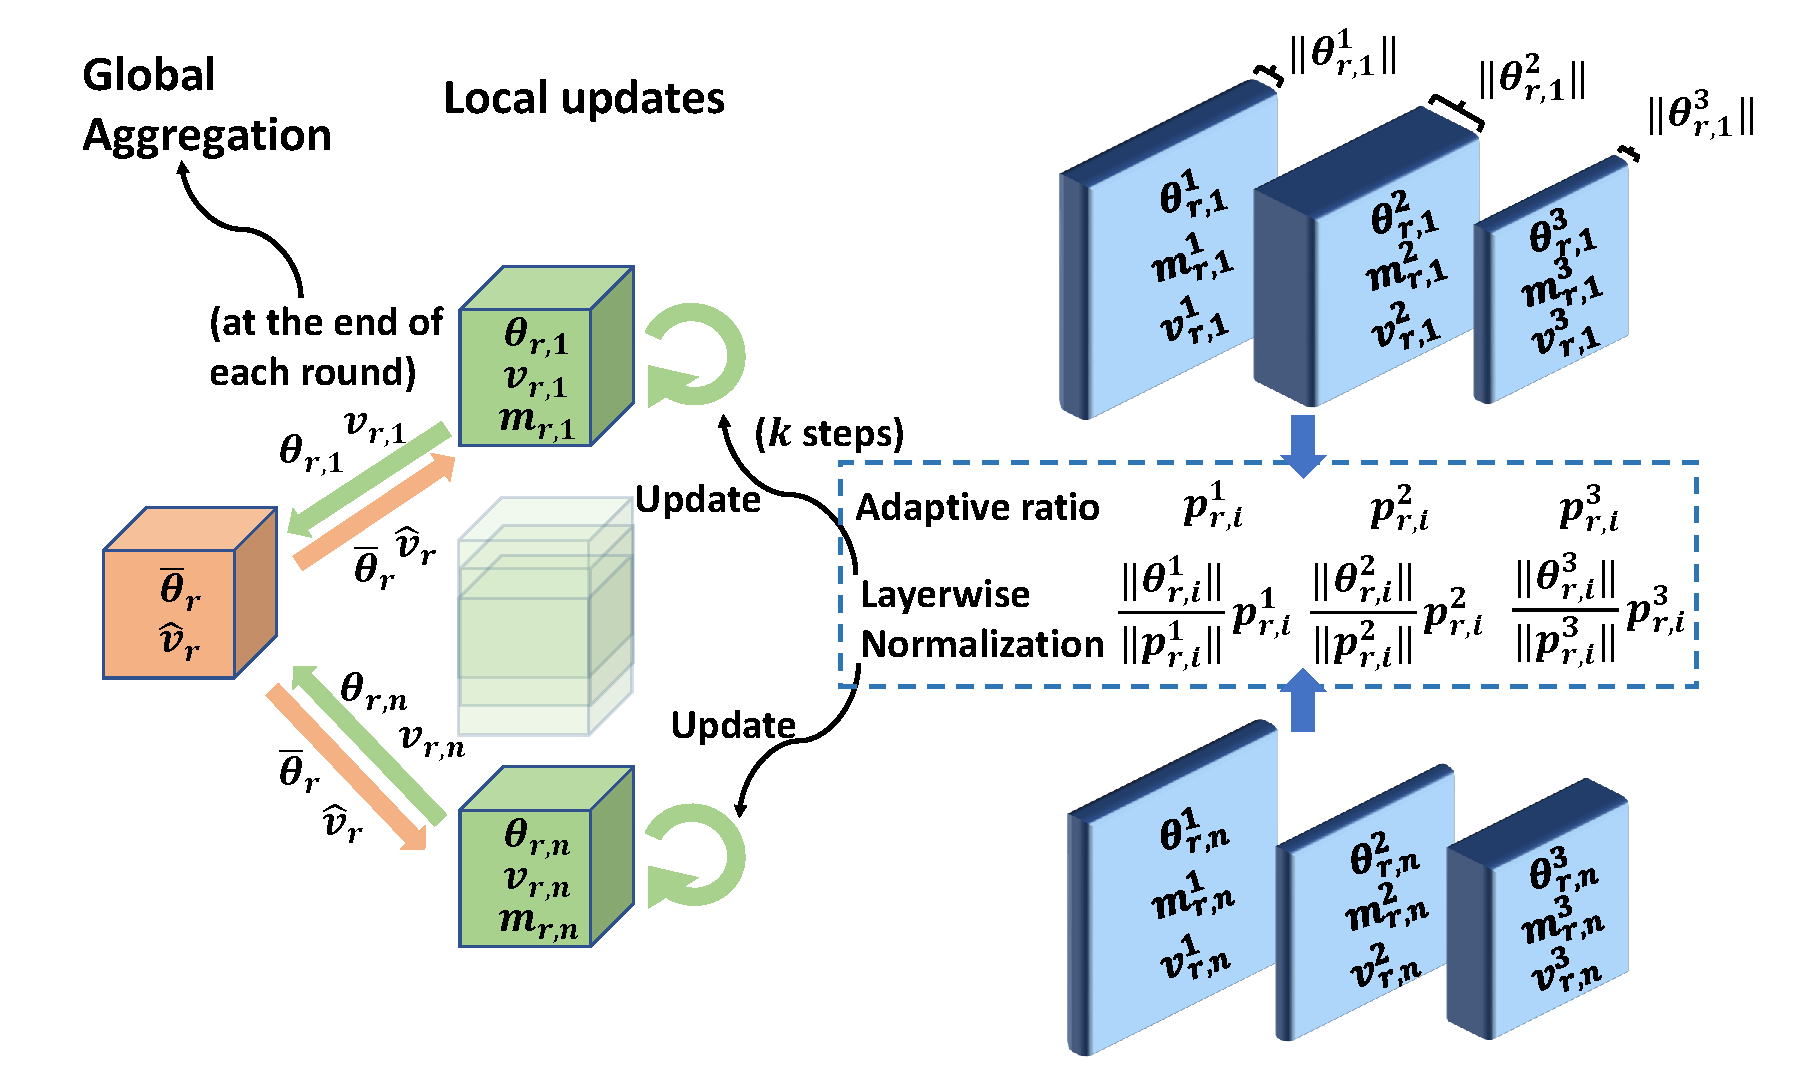
\includegraphics[width=0.4\textwidth]{new_figure/plot1.pdf}
}
	\caption{Illustration of Fed-LAMB (Algorithm~\ref{alg:ldams}), with a three-layer network and $\phi(x)=x$ as an example. %	The depth of each network layer represents the norm of its weights. 
		For device $i$ and each local iteration in round $r$, the adaptive ratio of $j$-th layer $p_{r,i}^j$ is normalized according to $\Vert \theta_{r,i}^j\Vert$, and then used for updating the local model. 
	At the end of each round $r$, local worker $i$ sends $\theta_{r,i} =  [\theta_{r,i}^{\ell}]_{\ell =1}^{\tot}$ and $v_{r,i}$ to the central server, which transmits back aggregated $\theta$ and $\hat v$ to local devices to complete a round of training.}
	\label{fig:illustrate}
\end{figure}




\vspace{0.2in}
\section{On The Convergence of \algo}\label{sec:theory}
We develop in this section, the theoretical analysis of Algorithm~\ref{alg:ldams}.  Based on classical result for stochastic nonconvex optimization, we provide a collection of results that aims to providing a better understanding of the convergence behavior of our distributed optimization method under the federated learning framework.
The main challenges we ought to overcome are manifold 
(i) The large amount of decentralized workers working solely on their own data stored locally. 
(ii) A periodic averaging occurs on the central server pushing each of those clients to send local models after some local iterations. 
(iii) Each client computes a backpropagation of the main model, i.e., the deep neural network, and then updates its local version of the model via an adaptive gradient method: the distinctiveness being that those updates are done \emph{dimensionwise} and \emph{layerwise}.
Our analysis encompasses the consideration of those challenges and leads to a informative convergence rates depending on the quantities of interest in our problem: the number of layers of the DNN, the number of communications rounds and the number of clients used under our federated settings.

\subsection{Finite Time Analysis of \algo}
In the sequel, the analysis of our scheme we provide is \emph{global}, in the sense that it does not depend on the initialization of our algorithm, and \emph{finite-time}, meaning that it is true for any arbitrary number of communication rounds, in particular small ones.
In the particular context of nonconvex stochastic optimization for distributed clients, we assume the following:

\vspace{0.1in}

\begin{assumption}\label{ass:smooth}(Smoothness per layer)
For $i \in \inter$ and $\ell \in \interl$: $\norm{\nabla f_i (\theta^\ell) - \nabla f_i (\vartheta^\ell)} \leq L_\ell \norm{\theta^\ell-\vartheta^\ell}$.
\end{assumption}
We add some classical assumption on the gradient of the objective function:
\begin{assumption}\label{ass:boundgrad}(Unbiased and Bounded gradient)
The stochastic gradient is unbiased for any iteration $r>0$: $\EE[g_r] = \nabla f(\theta_r)$ and is bounded from above, i.e., $\norm{g_t} \leq M$.
\end{assumption}

\begin{assumption}\label{ass:var}(Bounded variance)
The variance of the stochastic gradient is bounded for any iteration $r>0$ and any dimension $j \in \llbracket d \rrbracket$: $\EE[|g_r^j - \nabla f(\theta_r)^j|^2] < \sigma^2$.
\end{assumption}

\begin{assumption}\label{ass:phi}(Bounded Scale)
For any $a \in \rset^*_+$, there exists strictly positive constants such that $\phi_m \leq  \phi(a) \leq \phi_M$.
\end{assumption}



Two important Lemmas are required in the proof of the Theorem above.
We also report the complete proof of our bound in the Appendix of this paper.

The first result gives a characterization of the gap between the averaged model, that is computed by the central server in a periodic manner, and each of the local models stored in each client $i \in \inter$.
\begin{Lemma}\label{lemma:iterates}
Consider $\{\overline{\theta_r}\}_{r>0}$, the sequence of parameters obtained running Algorithm~\ref{alg:ldams}. Then for $i \in \inter$ and $r > 0$, the gap $\| \overline{\theta_r} - \theta_{r,i} \|^2$ satisfies:
\beq\notag
\| \overline{\theta_r} - \theta_{r,i} \|^2 \leq \alpha_r^2 M^2 \phi_M^2 \frac{(1-\beta_2)p}{v_0} \, ,
\eeq
where $\phi_M$ is defined in H\ref{ass:phi} and p is the total number of dimensions $p = \sum_{\ell = 1}^\tot p_\ell$.
\end{Lemma}

The gap is provably bounded by some quantities of interest such as the total dimension of the multilayered model $p$, the learning rate and the assumed upper bound of the  gradient, see H\ref{ass:boundgrad}.

Then, the following Lemma allows us to convert the suboptimality condition $\left\| \frac{\overline{\nabla}f(\theta_r)}{\sqrt{ v_r^t}} \right\|$ to the desired one which is $\left\| \frac{\nabla f(\overline{\theta_r})}{\sqrt{ v_r^t}} \right\|$.
Note that the end goal is to characterize how fast the gradient of the averaged/global parameter $\overline{\theta_r}$ goes to zero, and not the averaged gradient.



\begin{Lemma}\label{lemma:ratio}
Consider $\{\overline{\theta_r}\}_{r>0}$, the sequence of parameters obtained running Algorithm~\ref{alg:ldams}. Then for $r > 0$:
\beq\notag
\left\| \frac{\overline{\nabla}f(\theta_r)}{\sqrt{ v_r^t}} \right\|^2 \geq \frac{1}{2} \left\| \frac{\nabla f(\overline{\theta_r})}{\sqrt{ v_r^t}} \right\|^2 - \overline{L} \alpha^2 M^2 \phi_M^2 \frac{(1-\beta_2)p}{v_0}\, ,
\eeq
where $M$ is defined in H\ref{ass:boundgrad}, $p = \sum_{\ell = 1}^\tot p_\ell$ and $\phi_M$ is defined in H\ref{ass:phi}.
\end{Lemma}


We now state our main result regarding the non asymptotic convergence analysis of our Algorithm~\ref{alg:ldams} for multiple local updates and true for any communication rounds number $R$.



\begin{Theorem}\label{th:multiple update}
Assume \textbf{H\ref{ass:smooth}-H\ref{ass:phi}}. Consider $\{\overline{\theta_r}\}_{r>0}$, the sequence of parameters obtained running Algorithm~\ref{alg:ldams} with a constant learning rate $\alpha$. Let the number of local epochs be $T \geq 1$ and $\lambda = 0$. Then, for any round $R > 0$, we have
{\small
\beq \label{bound1multiple}
\begin{split}
&  \frac{1}{R}\sum_{r=1}^R  \EE\left[ \left\| \frac{\nabla f(\overline{\theta_t})}{\hat v_t^{1/4}}   \right \|^2 \right] \leq    \sqrt{\frac{M^2 p}{n}}  \frac{ \EE[f(\bar{\theta}_1)]  - \min \limits_{\theta \in \Theta} f(\theta)}{\tot \alpha R}\\
  &   +4\alpha \left[ \frac{\alpha^2 L_\ell}{\sqrt{v_0}} M^2 (T-1)^2 \phi_M^2 (1-\beta_2)p +\phi_M^2\sqrt{M^2+p\sigma^2} \right]  \\
    & +4\alpha \frac{M^2}{\sqrt{v_0}} +      \frac{\phi_M   \sigma^2}{R n} \sqrt{\frac{1 - \beta_2}{M^2 p}  } +4\alpha \left[\phi_M \frac{\tot \sigma^2}{\sqrt{n}}\right]   + cst. 
   \end{split}
\eeq
}

\end{Theorem}

By choosing a suitable learning rate, we have the following simplified result.
\begin{Corollary}\label{coro:main}
Under the same setting as Theorem~\ref{th:multiple update}, with $\alpha = \mathcal{O}(\frac{1}{ \sqrt{\tot R}})$, it holds that
{\small
\begin{align} \label{coro:rate}
&    \frac{1}{R}\sum_{r=1}^R  \EE\left[ \left\| \frac{\nabla f(\overline{\theta_t})}{\hat v_t^{1/4}}   \right \|^2 \right]\\
& \leq \mathcal{O}\left( \sqrt{\frac{ p}{n}} \frac{1}{\sqrt{\tot R}} + \frac{\sigma^2 }{R n\sqrt{p}}+\frac{(T-1)^2p}{\tot^3 R^{3/2}}\right).\notag
\end{align}
}
\end{Corollary}

%We recall that a $\epsilon-$stationary point is defined by the number of communication rounds $R$ such that $\frac{1}{R}\sum_{t=1}^\mathcal{R}  \EE\left[ \left\| \frac{\nabla f(\overline{\theta_t})}{\hat v_t^{1/4}}   \right \|^2 \right] \leq \epsilon$.


%\begin{Theorem}\label{th:main}
%Assume \textbf{H\ref{ass:smooth}-H\ref{ass:phi}}. Consider $\{\overline{\theta_r}\}_{r>0}$, the sequence of parameters obtained via Algorithm~\ref{alg:ldams} with a decreasing lr $\alpha_r$. Then, if $T=1$ and $\lambda = 0$:
%%\beq \label{bound1}
%%\begin{split}
%%  \frac{1}{R}\sum_{r=1}^R  \EE\left[ \left\| \frac{\nabla f(\overline{\theta_r})}{\sqrt{ v_r^t}}   \right \|^2 \right] 
%%   \leq &  \sqrt{\frac{M^2 p}{n}} \frac{ \EE[f(\bar{\theta}_1)]  - \min \limits_{\theta \in \Theta} f(\theta)}{\tot \alpha_r R}+      \frac{\phi_M   \sigma^2}{R n} \sqrt{\frac{1 - \beta_2}{M^2 p}  } \\
%%  +& \alpha_r \phi_M \sigma \tot p \sqrt{n}+ \frac{ \overline{L}\beta_1^2\tot(1-\beta_2)M^2 \phi^2_M n}{2(1-\beta_1)^2 v_0}    \\
%% + &\frac{\alpha_r \beta_1}{1-\beta_1}  \sqrt{(1-\beta_2)p} \frac{\tot M^2}{\sqrt{v_0}} +\overline{L} \alpha_r^2 M^2 \phi_M^2 \frac{(1-\beta_2)p}{Rv_0} 
%%   \end{split}
%%\eeq
%\beq \label{bound1}
%\begin{split}
%  \frac{1}{R}\sum_{r=1}^R  \EE\left[ \left\| \frac{\nabla f(\overline{\theta_r})}{\sqrt{ v_r^t}}   \right \|^2 \right] 
%   \leq   \sqrt{\frac{M^2 p}{n}} \frac{ \EE[f(\bar{\theta}_1)]  - f^*}{\tot \alpha_r R} + \frac{\phi_M}{R} \left[ \frac{(1-\beta_2)\overline{L} \alpha_r^2 M^2 \phi_Mp}{v_0} +  \frac{ \sigma^2}{n} \sqrt{\frac{1 - \beta_2}{M^2 p}  }    \right]
%   \end{split}
%\eeq
%where $\overline{L} = \sum_{\ell=1}^\tot L_{\ell}$ is the sum of all smoothness constants, $\tot$ is the total number of layers and $f^* \eqdef \min \limits_{\theta \in \Theta} f(\theta)$.
%\end{Theorem}


\subsection{Comparisons}

We dedicate the following paragraph to a discussion on the bound derived above in comparison with known results most relevant to our interest in the literature.

\vspace{0.05in}
\textbf{LAMB bound in~\citet{you2019large}: }
We first start our discussion with the comparison of convergence rate of \algo\ with that of LAMB, Theorem 3 in~\citet{you2019large}. 
The convergence rates of \algo and LAMB differ in two ways: 
(i) First, note that the characterization, on the suboptimality, or convergence criterion, is given at the averaged parameters noted $\overline{\theta_r}$ due to our distributed settings. 
It is thus natural to consider the evolution of our objective function, precisely its gradient, evaluated at some global model values --as opposed to the outcome of a single step drift in the central server paradigm. 
Besides, for ease of interpretation, the LHS of~\eqref{bound1multiple} is summed over all rounds instead of a fictive random termination point. A simple calculation would lead to such characterization, found in several nonconvex stochastic optimization paper such as~\cite{ghadimi2013stochastic}.
(ii)  Assuming that the convergence criterion in both Theorems is of similar order (which happens for a large enough number of rounds), convergence rate of \algo\ displays a similar $\mathcal{O}(1/R)$ behaviour for the initialization term, meaning that, despite the distributed (federated) settings, our dimensionwise and layerwise method benefits from the double adaptivity phenomenon explained above and exhibited in the LAMB method of~\citep{you2019large}, performed under a central server setting.


\vspace{0.05in}
\textbf{Local-AMS bound in~\citet{chen2020toward}: }
We now discuss the similarities and differences between local-AMS, the distributed adaptive method developed in~\citet{chen2020toward}, and our \emph{layerwise federated} method, namely \algo.
We recall their main result under our notations:

\vspace{0.1in}

\begin{Theorem}[Theorem 5.1 in~\citet{chen2020toward}]
Under some regularity conditions on the local losses and similar assumption as ours, with $\alpha=\mathcal O(\sqrt{n}/\sqrt{Rp})$, Local-AMS has the following convergence rate:
{\small
\beq \notag
\begin{split}
 \frac{1}{R}\sum_{r=1}^R  \EE\left[ \left\| \frac{\nabla f(\overline{\theta_r})}{\sqrt{ v_r^t}}   \right \|^2 \right]     \leq  \mathcal O( \sqrt{\frac{p}{Rn}} (1+\sigma^2) +\frac{n(T-1)^2}{R} )
 \end{split}
\eeq
}
where $\epsilon$ corresponds to their initialization of the vector $\hat v_0$ and $L_{s}$ is the sum of the local smoothness constants.
\end{Theorem}

The first two terms of their results and ours, standard in convergence analysis, displays a dependence of the convergence rate on the initialization and the bounded variance assumption of the stochastic gradient, see H\ref{ass:var}. In general, when the number of rounds $R$ is sufficiently large, both rates are dominated by $\mathcal O(\frac{\sqrt p}{\sqrt{n R}})$, matching the convergence rate of AMSGrad (e.g.~\cite{Arxiv:Zhou_18}).
The acceleration of our layerwise scheme is exhibited in the $\mathcal O(1/(n R))$ term and the dependence on the number of layers $\mathcal O(1/(h^3 R^{3/2}))$ term. Note that the boundedness assumption is done on each dimension in H\ref{ass:var} and leads to a manifestation of the term $\sqrt{p}$ in both rates. This can be handled for simplicity and clarity of the results when H\ref{ass:var} is assumed globally.

In~\eqref{coro:rate}, the last term containing the number of local updates $T$ is small as long as $T\leq \mathcal O(\frac{R^{1/2}h^{5/4}}{(np)^{1/4}})$. 
Treating $p^{1/4}/h=\mathcal O(1)$, the result implies that we can get the same rate of convergence as vanilla AMSGrad, with $R/T\geq \mathcal{O}(R^{1/2}n^{1/4})$ rounds of communication. For Local-AMS, by similar argument we know that, it requires $\mathcal O(R^{3/4}n^{3/4})$ communication rounds. Thus, our result reduces the number of communication rounds needed to reach a $\epsilon$-stationary point compared with~\cite{chen2020toward}, hence improving the communication efficiency.


\subsection{Discussions}
To help understand \algo\, we provide the discussion on our bound in several aspects:

\medskip
\textbf{Communication Complexity:} The (sublinear) dependence on the number of communication rounds of our bound matches that of most recent methods in federated learning, see~\citet{karimireddy2019scaffold} developing SCAFFOLD, a solution to the problem posed by heterogeneity of the data in each client, and of~\cite{reddi2020adaptive}, adapting state of the art method in optimization, here ADAM, under the federated setting. 
Yet, contrary to SCAFFOLD, our method only sends bits once per communication round while SCAFFOLD needs to send two vectors, including an additional control variate term  from the clients to the central server.
Novelty in our bound occurs considering the sublinear dependence on the number of layer $\tot$ and the dependence on the total number of dimension of our problem $p$. For the latter, the dependency can be simplified with stronger assumption on the control of the variance of the stochastic gradient. For the former, 

\medskip
\textbf{Homogeneous and Heterogeneous Data:} A common assumption regarding the stochastic gradient, and its variance, considers an upper-bound of the global variance, in the sense that it applies to both the aggregated objective function~\eqref{eq:opt} and each of its local component. 
An alternative theoretical approach is to set apart a local variance for each local loss, and global variance for their sum, see~\citet{chen2020toward} for instance.
Heterogeneity is of utmost importance in FL since client may store radically different data points in local devices.
Existing methods can lead to poor convergence as detailed in~\citet{li2019federated,liang2019variance}. 
Improvements are proposed through the use of gradient tracking techniques performed locally as seen in~\citet{haddadpour2020federated,horvath2019stochastic,karimireddy2019scaffold}.

\medskip
\textbf{Dependence on the dimension $p$:} The $\sqrt p$ term appearing in our bound is due to the assumption on coordinate-wise bounded variance. One may instead assume a bounded total variance to remove this term. 
In practice, the dependence on the overall size of the vectors being transmitted back and forth from the central to the devices can be improved in various ways. Indeed, recent efficient techniques aim at reducing the number of bits communicated at each round through sketches or compression techniques, see for instance~\citet{haddadpour2020fedsketch,ivkin2019communication,li2019privacy} to name a few.
This can be a great addition to \algo, and is naturally compatible, but is not the main focus of our contribution.





\section{Numerical Experiments}\label{sec:numerical}

In this section, we conduct numerical experiments on various datasets and network architectures to testify the effectiveness of our proposed method in practice. Our main objective is to validate the benefit of dimensionwise adaptive learning when integrated with adaptive Fed-AMS.
We observe in the sequel that our method empirically confirms its edge in terms of convergence speed.
Basically, our proposed method reduces the number of rounds and thus the communication cost required to achieve similar stationary points than baseline methods. 




\vspace{0.1in}
\noindent\textbf{Settings.} In our experiment, we will evaluate three federated learning algorithms: 1) Fed-SGD, 2) Fed-AMS and 3) our proposed Fed-LAMB (Algorithm~\ref{alg:ldams}), where the first two serve as the baseline methods. For adaptive methods 2) and 3), we set $\beta_1=0.9$, $\beta_2=0.999$ as default and recommended~\citep{reddi2019convergence}. Regarding federated learning environment, we use 50 local workers with 0.5 participation rate. That means, we randomly pick half of the workers to be active for training in each round. To best accord with real scenarios where the local training batch size is usually limited, we set a relatively small local update batch size as 32. In each round, the training samples are allocated to the active devices, and one local epoch is finished after all the local devices run one epoch over their received samples by batch training. We test different number of local epochs in our experiments. For each dataset and number of local epochs, we tune the constant learning rate $\alpha$ for each algorithm over a fine grid in logarithm scale. For Fed-LAMB, the parameter $\lambda$ in Algorithm~\ref{alg:ldams} controlling the overall scale of the layerwise gradients is tuned from $\{0,0.01,0.1\}$. 
For each experiment, we use the identity function for $\phi(\cdot)$.
For each run, we take the model performance with the best $\alpha$ and $\lambda$. The reported results are averaged over three independent runs, each with same initialization for every method.

\vspace{0.1in}
\noindent\textbf{Models.} We test the performance of different federated learning algorithms on MNIST~\citep{lecun1998mnist} and CIFAR10~\citep{krizhevsky2009learning} image classification datasets. For MNIST, we apply 1) a simple multilayer perceptron (MLP), which has one hidden layer containing 200 cells with dropout; 2) Convolutional Neural Network (CNN), which has two max-pooled convolutional layers followed by a dropout layer and two fully-connected layers with 320 and 50 cells respectively. For CIFAR10, we implement: 1) a CNN with three convolutional layers followed by two fully-connected layers, and 2) a ResNet-9 model proposed by~\cite{Proc:He-resnet16}. 
For each, we use both iid and non-iid data.


\subsection{Comparison under iid settings}

In Figure~\ref{fig:iid}, we report the test accuracies of a Convolutional Neural Network trained on CIFAR-10 dataset, where the data is iid allocated among clients.
When we run 1 local epoch per device, we observe a clear advantage of \algo over Fed-AMS on both test accuracy and convergence speed.
Note that Fed-SGD again fails to achieve close performance as those two adaptive gradient methods. 
Increasing the number of local iterations in each device per communication round leads to similar observations: our newly introduced method, namely \algo, converges the fastest, with similar generalization error as Fed-AMS. 

\begin{figure}[t]
    \begin{center}
        \mbox{
        \hspace{-0.05in}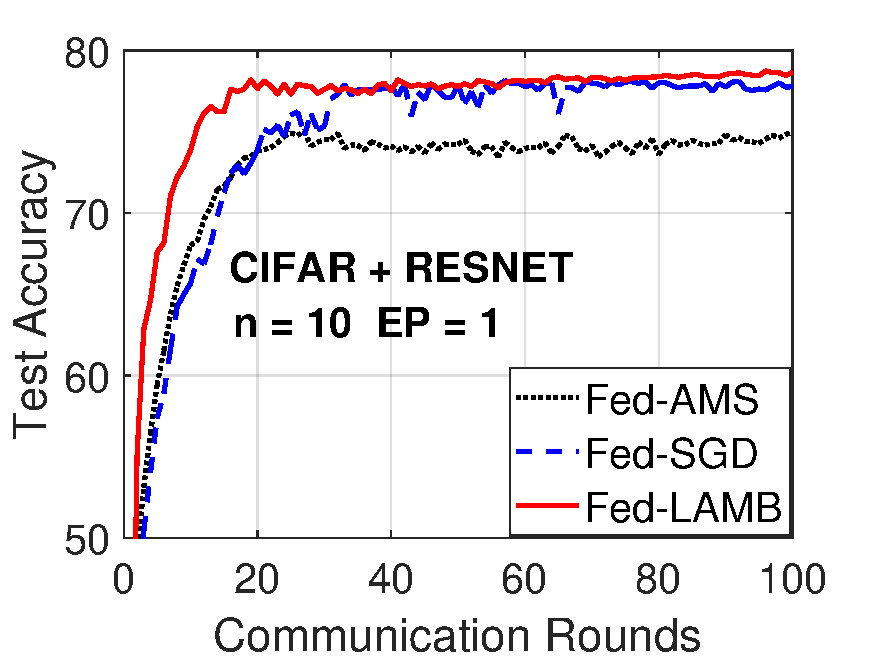
\includegraphics[width=0.25\textwidth]{new_figure/cifar_testerror_resnet_ep1_client10_iid1_SGD.pdf}
        \hspace{-0.1in} 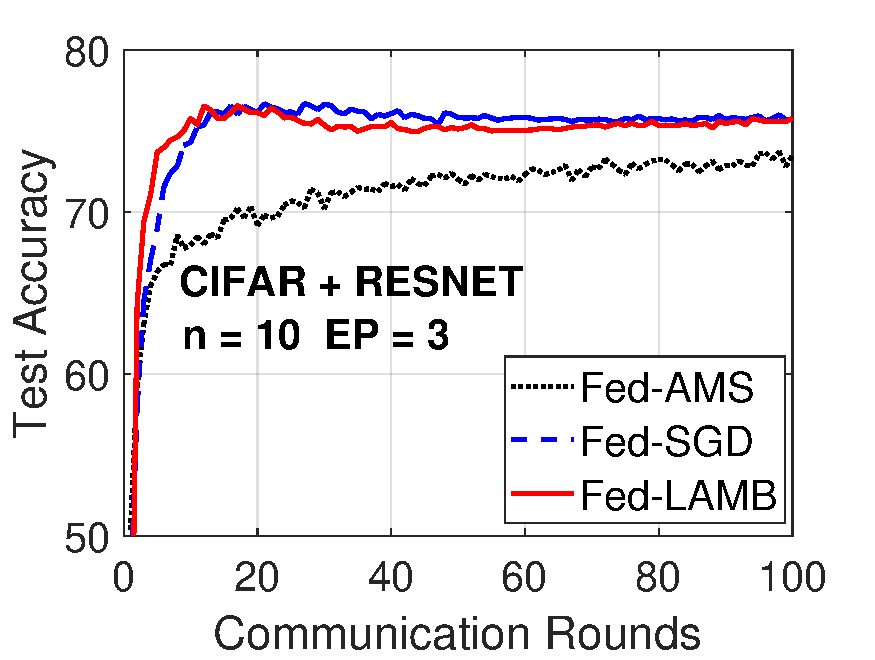
\includegraphics[width=0.25\textwidth]{new_figure/cifar_testerror_resnet_ep3_client10_iid1_SGD.pdf}
        }
        \mbox{
        \hspace{-0.05in}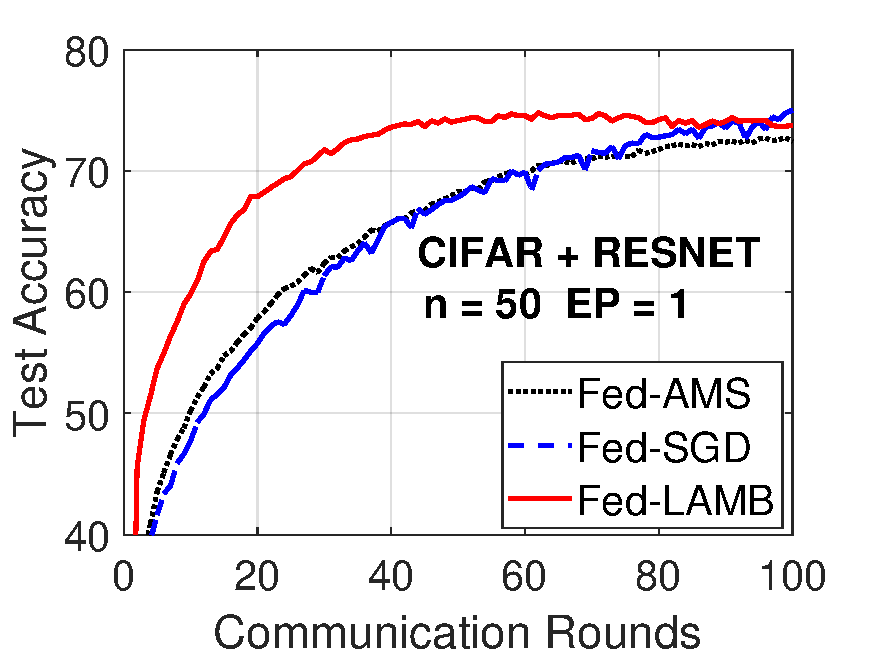
\includegraphics[width=0.25\textwidth]{new_figure/cifar_testerror_resnet_ep1_client50_iid1_SGD.pdf}
        \hspace{-0.1in}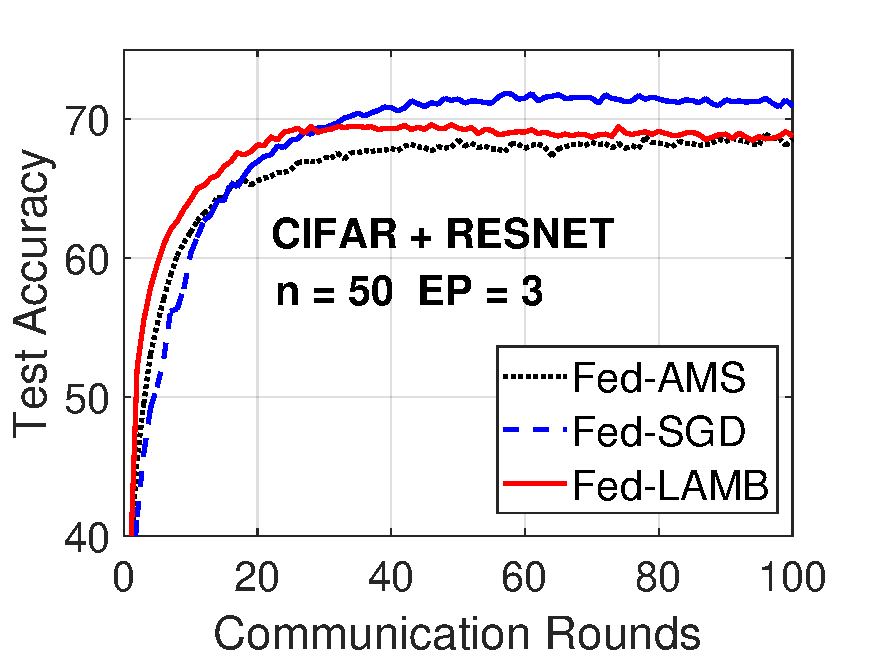
\includegraphics[width=0.25\textwidth]{new_figure/cifar_testerror_resnet_ep3_client50_iid1_SGD.pdf}
        }
        \mbox{        
        \hspace{-0.05in}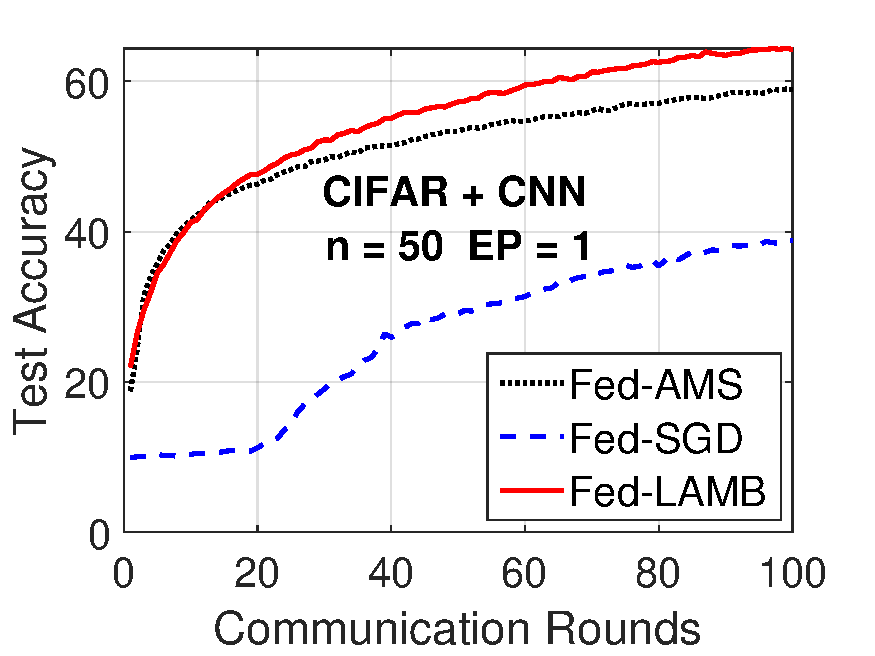
\includegraphics[width=0.25\textwidth]{new_figure/cifar_testerror_cnn_ep1_client50_iid1.pdf}
        \hspace{-0.1in}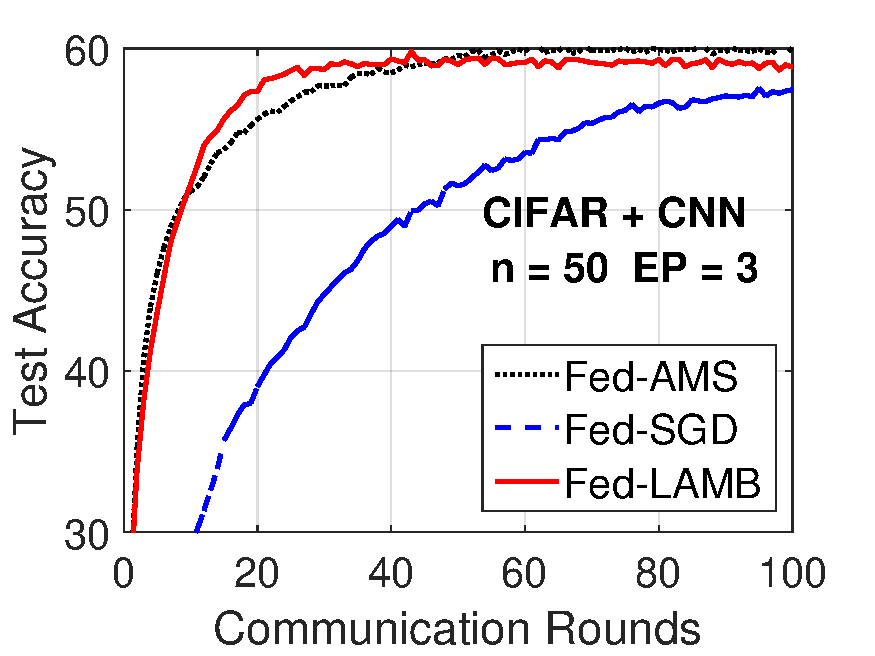
\includegraphics[width=0.25\textwidth]{new_figure/cifar_testerror_cnn_ep3_client50_iid1.pdf}
        }
    \end{center}
	\caption{\textbf{i.i.d. setting}. Top row: Test accuracy on CIFAR+ResNet, with iid data distribution for 10 clients. 
	{Middle row:} Test accuracy on CIFAR+ResNet with iid data distribution for 50 clients.
	{Bottom row:} Test accuracy on CIFAR+CNN with iid data distribution for 50 clients.
	\textbf{Left panel:} 1 local epoch. \textbf{Right panel:} 3 local epochs. 
	}
	\label{fig:iid}
\end{figure}



\subsection{Comparison under non-iid settings}

We then present Figure~\ref{fig:noniid}, the test accuracies on the MNIST and CIFAR dataset using either a MLP, CNN or ResNet-9 architecture. 
We compare each method under the heterogeneous (non-iid) data distribution settings, where each device only receives samples of one digit (out of ten). 
This is known to be the scenario where federated learning is harder to generalize well, see~\citet{mcmahan2017communication}. 
First of all, we observe that on MNIST using a simple MLP model, our proposed Fed-LAMB outperforms Fed-AMS and Fed-SGD with both 1 and 5 local epochs, illustrating its improvement over baseline federated methods. 
In addition, though it is not the main comparison of this paper, Fed-SGD slightly generalizes better than Fed-AMS, which means that SGD might be sufficient for this rather simple model. 
Yet, Fed-LAMB overachieves both methods on this task in terms of test accuracies.
Similar comparison can be drawn with respect to the training and testing losses.



\begin{figure}[t!]
    \begin{center}
        \mbox{
        \hspace{-0.05in}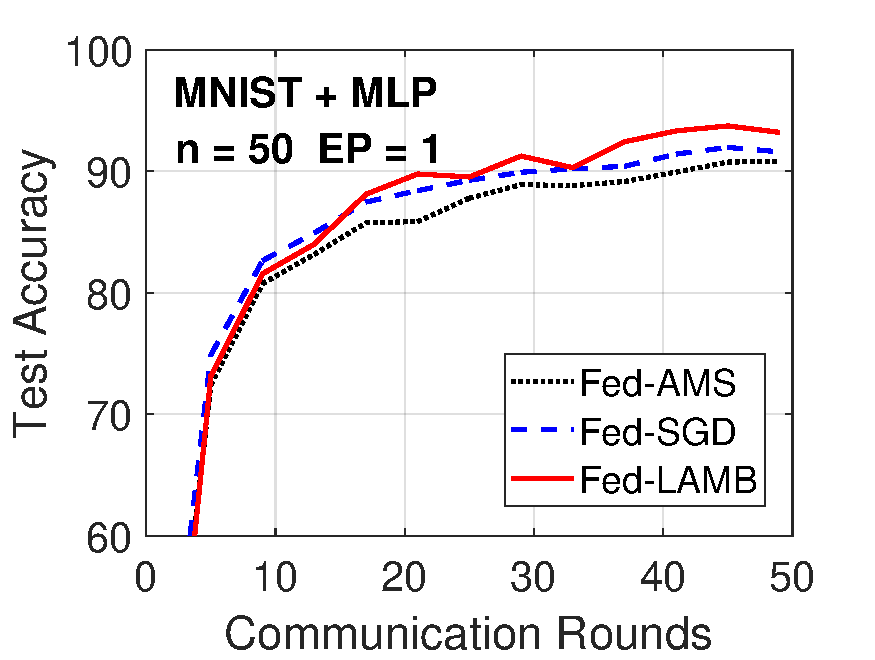
\includegraphics[width=0.25\textwidth]{new_figure/mnist_testerror_mlp_ep1_client50_iid0.pdf}
        \hspace{-0.1in}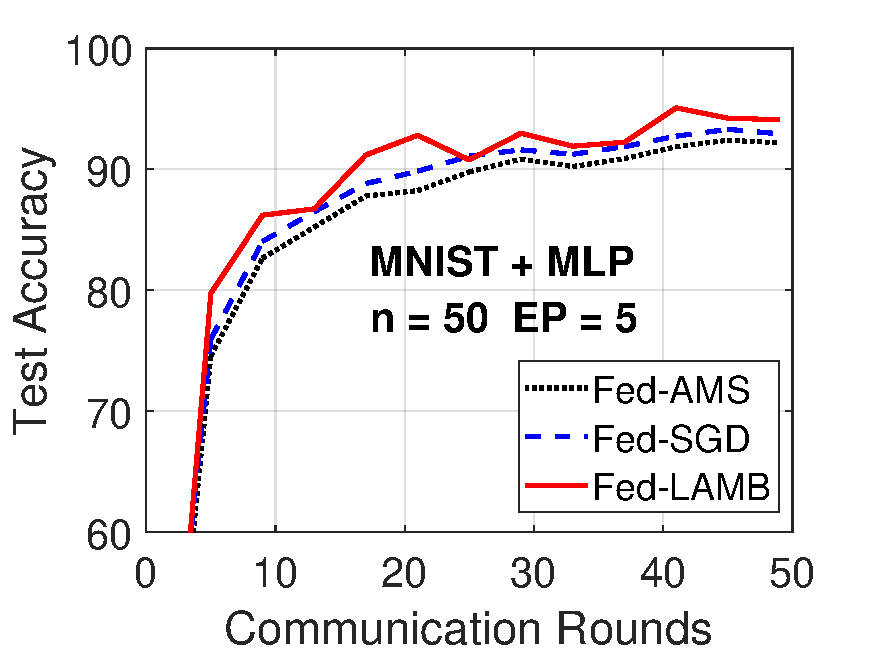
\includegraphics[width=0.25\textwidth]{new_figure/mnist_testerror_mlp_ep5_client50_iid0.pdf}
        }
        \mbox{
        \hspace{-0.05in}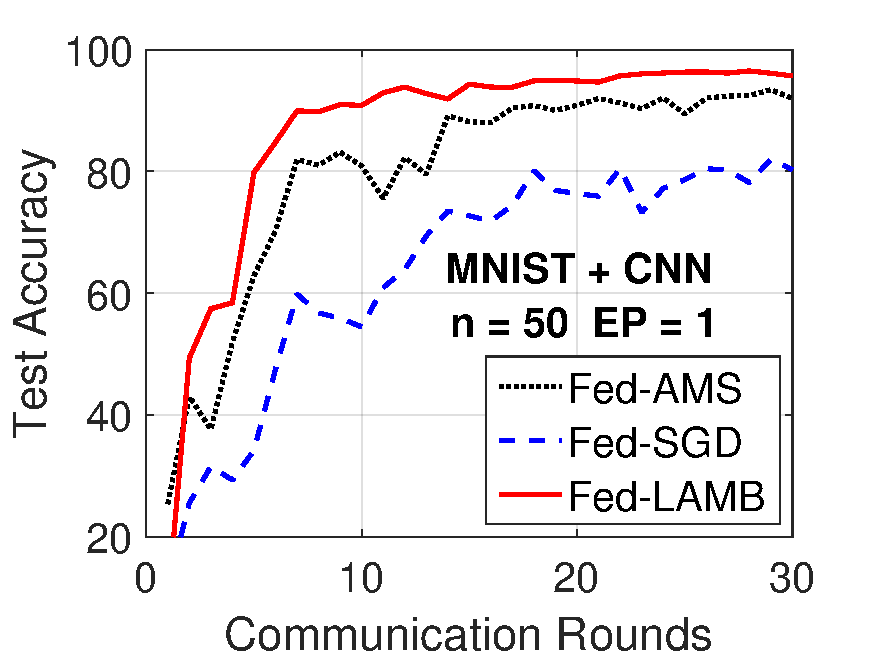
\includegraphics[width=0.25\textwidth]{new_figure/mnist_testerror_cnn_ep1_client50_iid0.pdf}
        \hspace{-0.1in}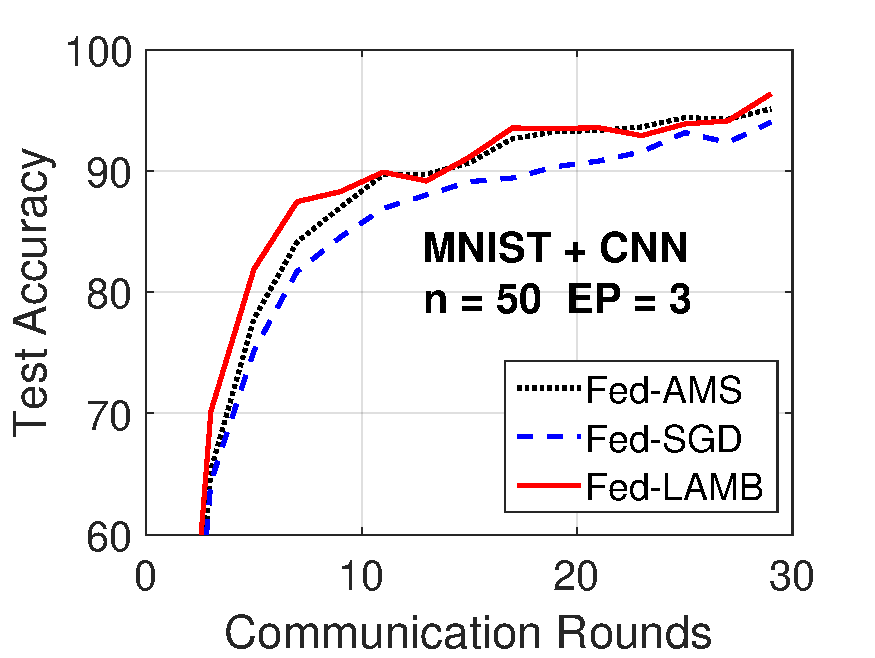
\includegraphics[width=0.25\textwidth]{new_figure/mnist_testerror_cnn_ep5_client50_iid0.pdf}
        }
        \mbox{
        \hspace{-0.05in}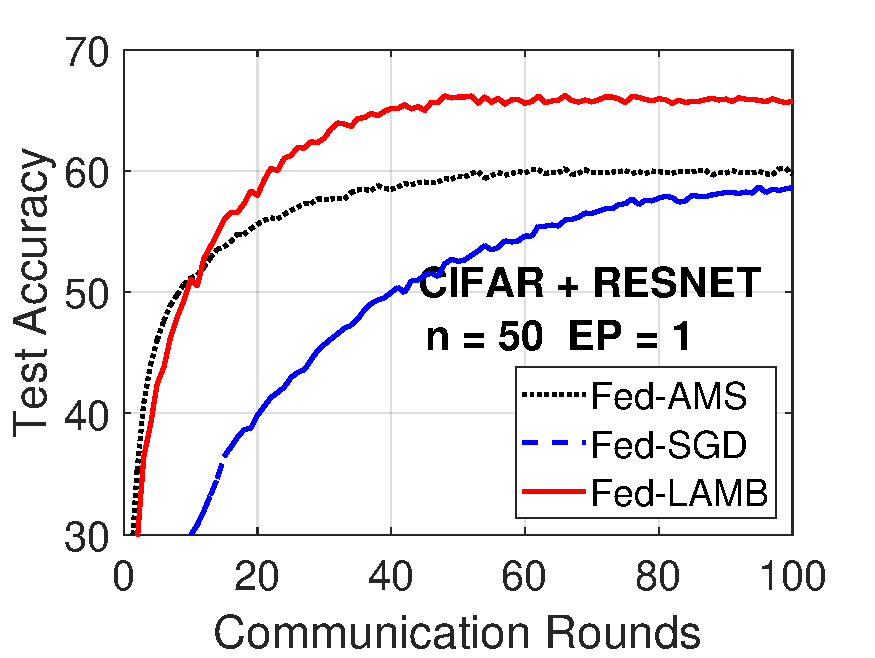
\includegraphics[width=0.25\textwidth]{new_figure/cifar_testerror_resnet_ep1_client50_iid0.pdf}
        \hspace{-0.1in}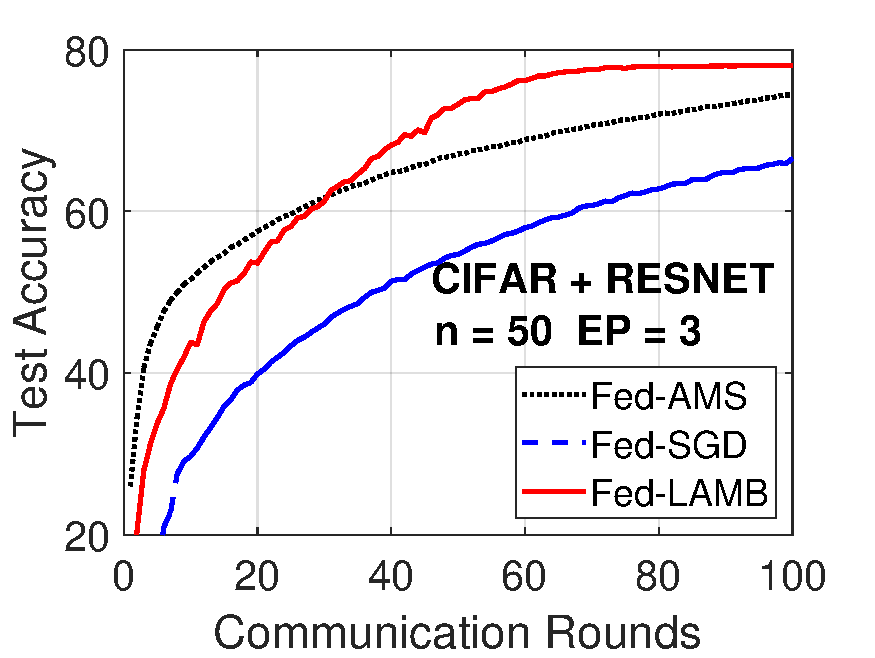
\includegraphics[width=0.25\textwidth]{new_figure/cifar_testerror_resnet_ep3_client50_iid0.pdf}        
        }
    \end{center}
	\caption{\textbf{non-i.i.d. setting.}. Top row: Test accuracy on MNIST+MLP, with non-iid data distribution. 
	{Middle row}: Test accuracy on MNIST+CNN, with non-iid data distribution. 
	{Bottom row:} Test accuracy on CIFAR+ResNet with non iid data distribution.
	\textbf{Left panel:} 1 local epoch. \textbf{Right panel:} 5 local epochs. 50 clients for each run.}
	\label{fig:noniid}
\end{figure}


We also evaluate various algorithms on larger models. 
Since Fed-LAMB is specifically designed for multi-layer deep learning networks, we expect it to show more substantial advantage over Fed-AMS on larger network architectures, since we recall that in Corollary~\ref{coro:main}, the convergence bound decreases with larger number of layers $\tot$.
For MNIST with CNN, under non-iid data distribution, we see that Fed-LAMB outperforms Fed-AMS in both cases. The advantage is in particular significant with 1 local epoch, where Fed-SGD generalizes poorly, see the left panel of Figure~\ref{fig:noniid}. 
Importantly, we would like to address the acceleration effect of Fed-LAMB, in the early stage of training. We observe that Fed-LAMB converges faster than the vanilla Fed-AMS at first few communication rounds, in both cases. 
As a side note, the poor performance of Fed-SGD is, to some extent, consistent with prior literature and practical numerical experiments showing that adaptive gradient methods usually perform better than simple SGD in training large deep learning models. We refer the readers to a collection of prior studies such as~\cite{chen2020toward,reddi2020adaptive}. 

Lastly, we test the algorithms on CIFAR-10 using a Residual Neural Network, the ResNet-9 model. 
We again observe in Figure~\ref{fig:noniid} that Fed-LAMB improves the performance of vanilla local AMS method under various settings regarding the number clients and number local iterations, corroborating the solid improvement brought by our laywerwise adaptive strategy. We see remarkable acceleration in the accuracy curve of Fed-LAMB, especially with 50 clients and 1 local epoch. In addition, Fed-AMS also compares favorably with Fed-SGD, though their performances are close on this specific task. 


\subsection{Comparison under non-iid settings and larger models}

We then present Figure~\ref{fig:noniidresnet18}, the test accuracies on the CIFAR and Tiny-ImageNet~\citep{le2015tiny} dataset using a ResNet-18 architecture. 

Here we adopt a a similar ResNet backbone model as above, now using 18 layers on Tiny-ImageNet which is a subset of ImageNet \citep{deng2009imagenet} and contains 200 classes, where each image is downsized to 64x64 pixels.

Figure~\ref{fig:noniidresnet18} displays how our layerwise and dimensionwise method behaves a) in the first epochs and b) at convergence best accuracy. We report the test accuracy for each baseline using 50 clients and one local epoch. We notice that while FedSGD is as fast as \algo on CIFAR10 using ResNet-18, our method leads to a better overall test accuracy ($92.43\%$ for \algo versus $90.76\%$ for FedSGD).
On Tiny-Imagenet, \algo shows great both non-asymptotic and asymptotic properties reaching an accuracy of $76.00\%$ after 100 communication rounds.


\begin{figure}[t!]
    \begin{center}
        \mbox{
        \hspace{-0.05in}\includegraphics[width=0.25\textwidth]{new_figure/cifar_testerror_resnet18_ep1_client2_iid0.eps}
        \hspace{-0.1in}\includegraphics[width=0.25\textwidth]{new_figure/tinyimagenet_testerror_resnet18_ep1_client2_iid0.eps}
        }
            \end{center}
	\caption{\textbf{non-i.i.d. setting.}. Test accuracy on CIFAR10+Resnet18 and TinyImagenet+Resnet18, with non-iid data distribution.
	}
	\label{fig:noniidresnet18}
\end{figure}




% \subsection{CIFAR-10 with Convolutional Neural Network and Residual  Network}

\section{Conclusion}\label{sec:conclusion}

We study in this contribution a doubly adaptive method in the particular framework of federated learning.
Built upon the success of periodic averaging, and of state-of-the-art adaptive gradient methods for single server nonconvex stochastic optimization, we derive \algo, a distributed AMSGrad method that performs local updates on each worker and periodically averages local models. 
Besides, when the trained model is a deep neural network, a core component of our method, namely \algo, is a \emph{layerwise} update of each local model.
The main contribution of our paper is thus a federated learning optimization algorithm that leverages a double level of adaptivity: the first one stemming from a \emph{dimensionwise} adaptivity of adaptive gradient methods, extended to their distributed (and local) counterpart, the second one is due to a  \emph{layerwise} adaptivity making use of the particular compositionality of the considered model.
Proved convergence guarantees of our scheme are provided in our contribution and exhibits a sublinear dependence on the total number of communications rounds, the number of clients and the number of layers of the model.
The multiple benefits of periodic averaging, adaptive optimization methods and layerwise updates are displayed in our bounds.
We empirically confirm the advantage of our algorithm over baselines methods on a panel of numerical experiments.
\clearpage

\bibliographystyle{plainnat}
\bibliography{ref}




\clearpage

\appendix 


\onecolumn

  \hsize\textwidth
  \linewidth\hsize  {\centering
  {\Large\bfseries Layerwise and Dimensionwise Locally Adaptive Optimization Method (Supplementary Material)\par}}
 
 \vspace{0.5in}
 
 
\textbf{Plan of the supplementary material:}
The supplementary material of this paper is composed of two main parts.
Section~\ref{app:proofs} contains detailed proofs of our results and Section~\ref{app:numericals} where additional runs are provided.
In particular, Theorem~\ref{th:multiple update} is proved in subsection~\ref{app:proofmain}.



\section{Theoretical Analysis}\label{app:proofs}

We first recall in Table~\ref{tab:notationsapp} some important notations that will be used in our following analysis.
\begin{table}[H]
%\caption{Table of Notations}
\begin{center}% used the environment to augment the vertical space
% between the caption and the table
\begin{tabular}{r c p{12cm} }
\toprule
$R, T$ & $\eqdef$ &  Number of communications rounds and local iterations (resp.)\\
$n, D, i$ & $\eqdef$ &  Total number of clients, portion sampled uniformly and client index \\
$\tot, \ell$ & $\eqdef$ &  Total number of layers in the DNN and its index \\
$\phi(\cdot)$ & $\eqdef$ &  Scaling factor in \algo update\\
$\bar{\theta}$ & $\eqdef$ &  Global model (after periodic averaging)\\
$p_{r,i}^{t}$ & $\eqdef$ &  ratio computed at round $r$, local iteration $t$ and for device $i$. $p_{r,i}^{\ell,t}$ denotes its component at layer $\ell$\\
\bottomrule
\end{tabular}
\end{center}
\caption{Summary of notations used in the paper.}
\label{tab:notationsapp}
\end{table}


We now provide the proofs for the theoretical results of the main paper, including the intermediary Lemmas and the main convergence result, Theorem~\ref{th:multiple update}.


\subsection{Intermediary Lemmas}


\begin{Lemma*}
Consider $\{\overline{\theta_r}\}_{r>0}$, the sequence of parameters obtained running Algorithm~\ref{alg:ldams}. Then for $i \in \inter$:
\beq\notag
\| \overline{\theta_r} - \theta_{r,i} \|^2 \leq \alpha^2 M^2 \phi_M^2 \frac{(1-\beta_2)p}{v_0} \eqsp,
\eeq
where $\phi_M$ is defined in H\ref{ass:phi} and p is the total number of dimensions $p = \sum_{\ell = 1}^\tot p_\ell$.
\end{Lemma*}

\begin{proof}
Assuming the simplest case when $T=1$, i.e. one local iteration, then by construction of Algorithm~\ref{alg:ldams}, we have for all $\ell \in \llbracket \tot \rrbracket$, $i \in \inter$ and $r >0$:
\beq\notag
 \theta^{\ell}_{r,i} =  \overline{\theta_r}^{\ell}  - \alpha \phi(\|\theta_{r,i}^{\ell,t-1}\|)p_{r,i}^{j} / \|p_{r,i}^{\ell}\|=  \overline{\theta_r}^{\ell}  - \alpha \phi(\|\theta_{r,i}^{\ell,t-1}\|)  
 \frac{m^{t}_{r,i}}{\sqrt{v^{t}_{r}}} \frac{1}{\|p_{r,i}^{\ell}\|}
\eeq
leading to 
\beq\notag
\begin{split}
\|\overline{\theta_r}   -  \theta_{r,i}\|^2 & = \sum_{\ell=1}^\tot \pscal{\overline{\theta_r}^{\ell}   -  \theta^{\ell}_{r,i}}{\overline{\theta_r}^{\ell}   -  \theta^{\ell}_{r,i}} \\
& \leq \alpha^2 M^2 \phi_M^2 \frac{(1-\beta_2)p}{v_0} \eqsp,
\end{split}
\eeq
which concludes the proof.
\end{proof}



\begin{Lemma*}
Consider $\{\overline{\theta_r}\}_{r>0}$, the sequence of parameters obtained running Algorithm~\ref{alg:ldams}. Then for $r > 0$:
\beq\notag
\left\| \frac{\overline{\nabla}f(\theta_r)}{\sqrt{ v_r^t}} \right\|^2 \geq \frac{1}{2} \left\| \frac{\nabla f(\overline{\theta_r})}{\sqrt{ v_r^t}} \right\|^2 - \overline{L} \alpha^2 M^2 \phi_M^2 \frac{(1-\beta_2)p}{v_0}
\eeq
where $M$ is defined in H\ref{ass:boundgrad}, p is the total number of dimensions $p = \sum_{\ell = 1}^\tot p_\ell$ and $\phi_M$ is defined in H\ref{ass:phi}.
\end{Lemma*}

\begin{proof}
Consider the following sequence:
\beq\notag
\begin{split}
\left\| \frac{\overline{\nabla}f(\theta_r)}{\sqrt{ v_r^t}} \right\|^2 \geq \frac{1}{2} \left\| \frac{\nabla f(\overline{\theta_r})}{\sqrt{ v_r^t}} \right\|^2 - \left\| \frac{\overline{\nabla}f(\theta_r)- \nabla f(\overline{\theta_r})}{\sqrt{ v_r^t}} \right\|^2 \eqsp,
\end{split}
\eeq
where the inequality is due to the Cauchy-Schwartz inequality.

Under the smoothness assumption H\ref{ass:smooth} and using Lemma~\ref{lemma:iterates}, we have
\beq\notag
\begin{split}
\left\| \frac{\overline{\nabla}f(\theta_r)}{\sqrt{ v_r^t}} \right\|^2 & \geq \frac{1}{2} \left\| \frac{\nabla f(\overline{\theta_r})}{\sqrt{ v_r^t}} \right\| - \left\| \frac{\overline{\nabla}f(\theta_r)- \nabla f(\overline{\theta_r})}{\sqrt{ v_r^t}} \right\|^2\\
& \geq \frac{1}{2} \left\| \frac{\nabla f(\overline{\theta_r})}{\sqrt{ v_r^t}} \right\|^2 - \overline{L} \alpha^2 M^2 \phi_M^2 \frac{(1-\beta_2)p}{v_0} \eqsp,
\end{split}
\eeq

which concludes the proof.
\end{proof}



\subsection{Proof of Theorem~\ref{th:multiple update}} \label{app:proofmain}



We now develop a proof for the two intermediary lemmas, Lemma~\ref{lemma:iterates} and Lemma~\ref{lemma:ratio}, in the case when each local model is obtained after more than one local update.
Then the two quantities, either the gap between the periodically averaged parameter and each local update, \ie $\| \overline{\theta_r} - \theta_{r,i} \|^2$, and the ratio of the average gradient, more particularly its relation to the gradient of the average global model (\ie $\left\| \frac{\overline{\nabla}f(\theta_r)}{\sqrt{ v_r^t}} \right\|$ and $ \left\| \frac{\nabla f(\overline{\theta_r})}{\sqrt{ v_r^t}} \right\| $), are impacted.

\begin{Theorem*}
Assume \textbf{H\ref{ass:smooth}-H\ref{ass:phi}}. Consider $\{\overline{\theta_r}\}_{r>0}$, the sequence of parameters obtained running Algorithm~\ref{alg:ldams} with a decreasing learning rate $\alpha$. Let the number of local epochs be $T \geq 1$ and $\lambda = 0$. Then, at iteration $\tau$, we have:
\beq \notag
\begin{split}
&  \frac{1}{\tau}\sum_{t=1}^\tau  \EE\left[ \left\| \frac{\nabla f(\overline{\theta_t})}{\hat v_t^{1/4}}   \right \|^2 \right] \leq    \sqrt{\frac{M^2 p}{n}}  \frac{ \EE[f(\bar{\theta}_1)]  - \min \limits_{\theta \in \Theta} f(\theta)}{\tot \alpha_r \tau} +      \frac{\phi_M   \sigma^2}{\tau n} \sqrt{\frac{1 - \beta_2}{M^2 p}  } \\
    &   +4\alpha \left[ \frac{\alpha^2 L_\ell}{\sqrt{v_0}} M^2 (T-1)^2 \phi_M^2 (1-\beta_2)p + \frac{M^2}{\sqrt{v_0}}+\phi_M^2\sqrt{M^2+p\sigma^2} + \phi_M \frac{\tot \sigma^2}{\sqrt{n}}\right]   + cst. \\
   \end{split}
\eeq
% If one considers a deceasing stepsize as  $\alpha_\tau = \mathcal{O}(\frac{1}{L \sqrt{\tau}})$, then:
% \begin{align}\notag
%     \frac{1}{\tau}\sum_{t=1}^\tau  \EE\left[ \left\| \frac{\nabla f(\overline{\theta_t})}{\hat v_t^{1/4}}   \right \|^2 \right] \leq \mathcal{O}\left( \sqrt{\frac{M^2 p}{n}} \frac{1}{\sqrt{\tot \tau}} + \frac{\sigma^2 }{\tau n\sqrt{p}}+\frac{(T-1)^2p}{\tau^{3/2}L^3}\right)
% \end{align}
\end{Theorem*}
% \textbf{Discussion on the bound:} Obviously, the last term containing the number of local updates $T$ is small as long as $T\leq \mathcal O(\frac{\tau^{1/2}L^{5/4}}{(np)^{1/4}})$. 
% Treating $p^{1/4}/L=\mathcal O(1)$ which is usually small, the result implies that we can get the same rate of convergence as the algorithm using one local update, with $\mathcal \mathcal{O}(\tau^{1/2}/n^{1/4})$ rounds of communication. 
% When the number of workers $n$ increases, then a constraint on the number of local updates $T$ is occurring, meaning that we would need more rounds of communication to achieve the same convergence rate, for a identical $\epsilon-$stationary point.
% We recall that a $\epsilon-$stationary point is defined by the number of communication rounds $\mathcal{R}$ such that $\frac{1}{\tau}\sum_{t=1}^\mathcal{R}  \EE\left[ \left\| \frac{\nabla f(\overline{\theta_t})}{\hat v_t^{1/4}}   \right \|^2 \right] \leq \epsilon$.

% We now provide the proof for Theorem~\ref{th:multiple update}.

\begin{proof}
Using H\ref{ass:smooth}, we have:
\begin{align}\notag
f(\bar{\vartheta}_{r+1}) &  \leq f(\bar{\vartheta}_r) + \pscal{\nabla f(\bar{\vartheta}_r)}{\bar{\vartheta}_{r+1} - \bar{\vartheta}_r} + \sum_{\ell =1}^L \frac{L_\ell}{2} \| \bar{\vartheta}^\ell_{r+1} - \bar{\vartheta}^\ell_r \|^2\\\notag
&  \leq f(\bar{\vartheta}_r) + \sum_{\ell=1}^\tot \sum_{j=1}^{p_\ell} \nabla_{\ell} f(\bar{\vartheta}_r)^j (\bar{\vartheta}^{\ell,j}_{r+1} - \bar{\vartheta}^{\ell,j}_r) + \sum_{\ell =1}^L \frac{L_\ell}{2} \| \bar{\vartheta}^\ell_{r+1} - \bar{\vartheta}^\ell_r \|^2  \eqsp.
\end{align}

Taking expectations on both sides leads to:
\begin{align}\label{eq:main}
- \EE[  \pscal{\nabla f(\bar{\vartheta}_r)}{\bar{\vartheta}_{r+1} - \bar{\vartheta}_r}]  \leq  \EE[ f(\bar{\vartheta}_r) - f(\bar{\vartheta}_{r+1})] + \sum_{\ell =1}^L \frac{L_\ell}{2} \EE[  \| \bar{\vartheta}^\ell_{r+1} - \bar{\vartheta}^\ell_r \|^2] \eqsp.
\end{align}

Yet, we observe that, using the classical intermediate quantity, used for proving convergence results of adaptive optimization methods, see for instance~\citep{RKK18}, we have:
\beq\label{eq:defseq}
\bar{\vartheta}_r = \bar{\theta}_r +  \frac{\beta_1}{1-\beta_1}(\bar{\theta}_{r} - \bar{\theta}_{r-1}) \eqsp,
\eeq
where $\bar{\theta_r}$ denotes the average of the local models at round $r$.
Then for each layer $\ell$,
\begin{align}\label{eq:gap}
\bar{\vartheta}^\ell_{r+1} - \bar{\vartheta}^\ell_r  & = \frac{1}{1-\beta_1}(\bar{\theta}^\ell_{r+1} - \bar{\theta}^\ell_{r}) - \frac{\beta_1}{1-\beta_1}(\bar{\theta}^\ell_{r} - \bar{\theta}^\ell_{r-1})\\
& = \frac{\alpha_{r}}{1-\beta_1} \frac{1}{n} \sum_{i = 1}^n \frac{\phi(\|\theta_{r,i}^{\ell}\|)}{\|p_{r,i}^{\ell}\|} p_{r,i}^{\ell}  - \frac{\alpha_{r-1}}{1-\beta_1} \frac{1}{n} \sum_{i = 1}^n \frac{\phi(\|\theta_{r-1,i}^{\ell}\|)}{\|p_{r-1,i}^{\ell}\|} p_{r-1,i}^{\ell}\\
& = \frac{\alpha \beta_1}{1-\beta_1} \frac{1}{n}  \sum_{i = 1}^n  \left( \frac{\phi(\|\theta_{r,i}^{\ell}\|)}{\sqrt{v^{t}_{r}} \|p_{r,i}^{\ell}\|} - \frac{\phi(\|\theta_{r-1,i}^{\ell}\|)}{\sqrt{v^{t}_{r-1}} \|p_{r-1,i}^{\ell}\|} \right) m^{t}_{r-1} + \frac{\alpha}{n} \sum_{i = 1}^n \frac{\phi(\|\theta_{r,i}^{\ell}\|)}{\sqrt{v^{t}_{r}} \|p_{r,i}^{\ell}\|} g^t_{r,i} \eqsp,
\end{align}
where we have assumed a constant learning rate $\alpha$.


We note for all $\theta \in \Theta$, the majorant $G > 0$ such that $\phi(\|\theta \|) \leq G$. 
Then, following~\eqref{eq:main}, we obtain:
\begin{align}\label{eq:main2}
- \EE[  \pscal{\nabla f(\bar{\vartheta}_r)}{\bar{\vartheta}_{r+1} - \bar{\vartheta}_r}]  \leq  \EE[ f(\bar{\vartheta}_r) - f(\bar{\vartheta}_{r+1})] + \sum_{\ell =1}^L \frac{L_\ell}{2} \EE[  \| \bar{\vartheta}_{r+1} - \bar{\vartheta}_r \|^2] \eqsp.
\end{align}

Developing the LHS of~\eqref{eq:main2} using~\eqref{eq:gap} leads to

\begin{align}\label{eq:inner}
\pscal{\nabla f(\bar{\vartheta}_r)}{\bar{\vartheta}_{r+1} - \bar{\vartheta}_r} &= \sum_{\ell=1}^\tot \sum_{j=1}^{p_\ell} \nabla_{\ell} f(\bar{\vartheta}_r)^j (\bar{\vartheta}^{\ell,j}_{r+1} - \bar{\vartheta}^{\ell,j}_r) \\
& =  \frac{\alpha \beta_1}{1-\beta_1}\frac{1}{n}  \sum_{\ell=1}^\tot \sum_{j=1}^{p_\ell} \nabla_{\ell} f(\bar{\vartheta}_r)^j \left[   \sum_{i = 1}^n  \left( \frac{\phi(\|\theta_{r,i}^{\ell}\|)}{\sqrt{v^{t}_{r}} \|p_{r,i}^{\ell}\|} - \frac{\phi(\|\theta_{r-1,i}^{\ell}\|)}{\sqrt{v^{t}_{r-1}} \|p_{r-1,i}^{\ell}\|} \right) m^{t}_{r-1}  \right] \\
& \underbrace{ -\frac{\alpha}{n} \sum_{\ell=1}^\tot \sum_{j=1}^{p_\ell} \nabla_{\ell} f(\bar{\vartheta}_r)^j  \sum_{i = 1}^n \frac{\phi(\|\theta_{r,i}^{\ell}\|)}{\sqrt{v^{t}_{r}} \|p_{r,i}^{\ell}\|} g_{r,i}^{t,l,j}}_{= A_1}   \label{eqn1} \eqsp.
\end{align}



We change all index $r$ to iteration $t$. 
Suppose $T$ is the number of local iterations. We can write~\eqref{eqn1} as
\begin{align}\notag
    A_1=-\alpha_t \langle \nabla f(\bar \vartheta_t),\frac{\bar g_t}{\sqrt{\hat v_t}} \rangle,
\end{align}
where $\bar g_t=\frac{1}{n}\sum_{i=1}^n \bar g_{t,i}$, with $\bar g_{t,i}=\Big[\frac{\phi(\Vert \theta_{t,i}^1\Vert)}{\Vert p_{t,i}^1\Vert}g_{t,i}^1,..., \frac{\phi(\Vert \theta_{t,i}^L\Vert)}{\Vert p_{t,i}^L\Vert}g_{t,i}^L   \Big]$ representing the normalized gradient (concatenated by layers) of the $i$-th device. It holds that
\begin{align}
    \langle \nabla f(\bar \vartheta_t),\frac{\bar g_t}{\sqrt{\hat v_t}} \rangle&=\frac{1}{2}\Vert \frac{\nabla f(\bar\vartheta_t) }{\hat v_t^{1/4}}\Vert^2+\frac{1}{2}\Vert \frac{\bar g_t }{\hat v_t^{1/4}}\Vert^2-\Vert \frac{\nabla f(\bar\vartheta_t)-\bar g_t }{\hat v_t^{1/4}}\Vert^2.  \label{eqn:x1}
\end{align}
To bound the last term on the RHS, we have
\begin{align}\notag
    \Vert \frac{\nabla f(\bar\vartheta_t)-\bar g_t }{\hat v_t^{1/4}}\Vert^2&=\Vert \frac{\frac{1}{n}\sum_{i=1}^n (\nabla f(\bar\vartheta_t)-\bar g_{t,i})}{\hat v_t^{1/4}} \Vert^2\\\notag
    &\leq \frac{1}{n}\sum_{i=1}^n\Vert \frac{\nabla f(\bar\vartheta_t)-\bar g_{t,i}}{\hat v_t^{1/4}} \Vert^2\\\notag
    &\leq \frac{2}{n}\sum_{i=1}^n \Big(\Vert \frac{\nabla f(\bar\vartheta_t)-\nabla f(\bar\theta_t)}{\hat v_t^{1/4}} \Vert^2+\Vert \frac{\nabla f(\bar\theta_t)-\bar g_{t,i}}{\hat v_t^{1/4}} \Vert^2  \Big). 
\end{align}
By Lipschitz smoothness of the loss function, the first term admits
\begin{align}\notag
    \frac{2}{n}\sum_{i=1}^n\Vert \frac{\nabla f_i(\bar\vartheta_t)-\nabla f_i(\bar\theta_t)}{\hat v_t^{1/4}} \Vert^2&\leq \frac{2}{n \sqrt{v_0}}\sum_{i=1}^n L_\ell\Vert \bar\vartheta_t-\bar\theta_t\Vert^2  \\\notag
    &=\frac{2L_\ell}{n \sqrt{v_0}}\frac{\beta_1^2}{(1-\beta_1)^2}\sum_{i=1}^n \Vert \bar\theta_t-\bar\theta_{t-1}\Vert ^2\\\notag
    &\leq \frac{2\alpha_r^2 L_\ell }{n \sqrt{v_0}}\frac{\beta_1^2}{(1-\beta_1)^2} \sum_{l=1}^L \sum_{i=1}^n\Vert \frac{\phi(\Vert \theta_{t,i}^l\Vert)}{\Vert p_{t,i}^l\Vert}p_{t,i}^l \Vert^2\\\notag
    &\leq \frac{2\alpha_r^2 L_\ell p\phi_M^2}{ \sqrt{v_0}}\frac{\beta_1^2}{(1-\beta_1)^2}.
\end{align}
For the second term,
\begin{align}\label{eq:inter}
    \frac{2}{n}\sum_{i=1}^n\Vert \frac{\nabla f(\bar\theta_t)-\bar g_{t,i}}{\hat v_t^{1/4}} \Vert^2 \leq \frac{4}{n}\Big( \underbrace{\sum_{i=1}^n \Vert \frac{\nabla f(\bar\theta_t)-\nabla f(\theta_{t,i})}{\hat v_t^{1/4}} \Vert^2}_{B_1} + \underbrace{ \sum_{i=1}^n\Vert \frac{\nabla f(\theta_{t,i})-\bar g_{t,i}}{\hat v_t^{1/4}} \Vert^2}_{B_2} \Big).
\end{align}
Using the smoothness of $f_i$ we can transform $B_1$ into consensus error by
\begin{align}\notag
    B_1&\leq \frac{L}{\sqrt{v_0}}\sum_{i=1}^n \Vert \bar\theta_t - \theta_{t,i}\Vert^2  \label{eqn:B1}\\
    &=\frac{\alpha_r^2 L}{\sqrt{v_0}}\sum_{i=1}^n\sum_{l=1}^L \| \sum_{j=\lfloor t \rfloor_T+1}^t \Big( \frac{\phi(\Vert \theta_{j,i}^l\Vert)}{\Vert p_{j,i}^l\Vert}p_{j,i}^l-\frac{1}{n}\sum_{k=1}^n \frac{\phi(\Vert \theta_{j,k}^l\Vert)}{\Vert p_{j,k}^l\Vert}p_{j,k}^l \Big) \|^2\\\notag
    &\leq n \frac{\alpha_t^2 L}{\sqrt{v_0}} M^2 (T-1)^2 \phi_M^2 (1-\beta_2)p
\end{align}
where the last inequality stems from Lemma~\ref{lemma:iterates} in the particular case where $  \theta_{t,i}$ are averaged every $ct+1$ local iterations for any integer $c$, since $(t-1)-(\lfloor t \rfloor_T+1)+1 \leq T-1$.
% The expectation of $B_2$ relates to the variance and bias of the stochastic gradients,
% \begin{align}
%     \mathbb E[B_2]&=\mathbb E[\sum_{i=1}^n\Vert \frac{\nabla f(\theta_{t,i})-g_{t,i}+g_{t,i}-\bar g_{t,i}}{\hat v_t^{1/4}} \Vert^2] \\
%     &\leq \mathbb E[\sum_{i=1}^n \Vert \frac{\nabla f(\theta_{t,i})-g_{t,i}}{\hat v_t^{1/4}} \Vert^2+\Vert \frac{g_{t,i}-\bar g_{t,i}}{\hat v_t^{1/4}} \Vert^2]\\
%     &\leq \frac{np\sigma^2}{\sqrt{v_0}}+\frac{1}{\sqrt{v_0}}\mathbb E[\sum_{i=1}^n \sum_{l=1}^{\tot} \Vert (1-\frac{\phi(\|\theta_{t,i}^l \|)}{\| p_{t,i}^l \|})g_{t,i}^l \Vert^2]\\
%     &\leq \frac{np\sigma^2}{\sqrt{v_0}}+\frac{nM^2L\phi_M^2(1-\beta_2)}{p\sqrt{v_0}} (incorrect!),
% \end{align}


We now develop the expectation of $B_2$ under the simplification that $\beta_1 = 0$:
\begin{align}\notag
    \mathbb E[B_2]&=\mathbb E[\sum_{i=1}^n\Vert \frac{\nabla f(\theta_{t,i})-\bar g_{t,i}}{\hat v_t^{1/4}} \Vert^2] \\\notag
    &\leq \frac{nM^2}{\sqrt{v_0}}+n\phi_M^2\sqrt{M^2+p\sigma^2}-2\sum_{i=1}^n\mathbb E[\langle \nabla f(\theta_{t,i}),\bar g_{t,i} \rangle/\sqrt{\hat v_t}]\\\notag
    &=\frac{nM^2}{\sqrt{v_0}}+n\phi_M^2\sqrt{M^2+p\sigma^2}-2\sum_{i=1}^n \sum_{\ell=1}^L \mathbb E[\langle \nabla_\ell f(\theta_{t,i}),\frac{\phi(\|\theta_{t,i}^l \|)}{\| p_{t,i}^l \|}g_{t,i}^l \rangle/\sqrt{\hat v_t^l}]\\\notag
    &=\frac{nM^2}{\sqrt{v_0}}+n\phi_M^2\sqrt{M^2+p\sigma^2}-2\sum_{i=1}^n \sum_{l=1}^L\sum_{i=1}^{p_l} \mathbb E[\nabla_l f(\theta_{t,i})^j\frac{\phi(\|\theta_{t,i}^{l,j} \|)}{\sqrt{\hat v_t^{l,j}}\| p_{t,i}^{l,j} \|}g_{t,i}^{l,j} ]\\\notag
    & \leq \frac{nM^2}{\sqrt{v_0}}+n\phi_M^2\sqrt{M^2+p\sigma^2}-2\sum_{i=1}^n \sum_{l=1}^L\sum_{i=1}^{p_l} \mathbb E \left[ \sqrt{\frac{1-\beta_2}{M^2 p_\ell}}  \phi(\|\theta_{r,i}^{l,j}\|)  \nabla_l f(\theta_{t,i})^j  g_{t,i}^{l,j}\right]\\\notag
    &\hspace{0.4in} -2 \sum_{i = 1}^n \sum_{l=1}^L\sum_{j=1}^{p_l}  E \left[  \left( \phi(\|\theta_{r,i}^{l,j}\|)   \nabla_l f(\theta_{t,i})^j   \frac{g_{r,i}^{t,l,j}}{ \|p_{r,i}^{l,j}\|}\right)\mathsf{1}\left( \sign(  \nabla_l f(\theta_{t,i})^j \neq  \sign( g_{r,i}^{t,l,j}) \right)\right]
\end{align}
where we use assumption H\ref{ass:boundgrad}, H\ref{ass:var} and H\ref{ass:phi}. 
Yet,
\begin{align*}
&- \mathbb E \Bigg[  \left( \phi(\|\theta_{r,i}^{l,j}\|)   \nabla_l f(\theta_{t,i})^j   \frac{g_{r,i}^{t,l,j}}{ \|p_{r,i}^{l,j}\|}\right)\mathsf{1}\left( \sign(  \nabla_l f(\theta_{t,i})^j
\neq  \sign( g_{r,i}^{t,l,j}) \right)\Bigg] \\
&\hspace{2in} \leq  \phi_M \nabla_l f(\theta_{t,i})^j   \mathbb{P}\left[  \sign(  \nabla_l f(\theta_{t,i})^j \neq  \sign( g_{r,i}^{t,l,j}) \right]
\end{align*}
Then we have:
\begin{align}\notag
    \mathbb E[B_2]\leq  \frac{nM^2}{\sqrt{v_0}}+n\phi_M^2\sqrt{M^2+p\sigma^2}-2 \phi_m \sqrt{\frac{1-\beta_2}{M^2 p}} \sum_{i=1}^n \E[\| [\nabla f(\theta_{t,i}) \|^2] + \phi_M \frac{\tot \sigma^2}{\sqrt{n}}
\end{align}
Thus,~\eqref{eq:inter} becomes:
\begin{align}\notag
    \frac{2}{n}\sum_{i=1}^n\Vert \frac{\nabla f_i(\bar\theta_t)-\bar g_{t,i}}{\hat v_t^{1/4}} \Vert^2 \leq 4 \left[ \frac{\alpha_t^2 Ll}{\sqrt{v_0}} \alpha_r^2 M^2 (T-1)^2 \phi_M^2 (1-\beta_2)p + \frac{M^2}{\sqrt{v_0}}+\phi_M^2\sqrt{M^2+p\sigma^2} + \phi_M \frac{\tot \sigma^2}{\sqrt{n}}\right]
\end{align}

Substituting all ingredients into (\ref{eqn:x1}), we obtain
\begin{align}\notag
    -\alpha_t \mathbb E[\langle \nabla f(\bar \vartheta_t),\frac{\bar g_t}{\sqrt{\hat v_t}} \rangle] &\leq -\frac{\alpha_t}{2}\mathbb E\big[\Vert \frac{\nabla f(\bar\vartheta_t) }{\hat v_t^{1/4}}\Vert^2 \big]-\frac{\alpha_t}{2}\mathbb E\big[\Vert \frac{\bar g_t }{\hat v_t^{1/4}}\Vert^2 \big]+\frac{2\alpha_t^3 L_\ell p\phi_M^2}{ \sqrt{v_0}}\frac{\beta_1^2}{(1-\beta_1)^2} \\\notag
    &\hspace{0.4in}  + 4 \left[ \frac{\alpha_t^2 L}{\sqrt{v_0}} M^2 (T-1)^2 \phi_M^2 (1-\beta_2)p + \frac{M^2}{\sqrt{v_0}}+\phi_M^2\sqrt{M^2+p\sigma^2} + \phi_M \frac{\tot \sigma^2}{\sqrt{n}}\right].
\end{align}
At the same time, we have
\begin{align}\notag
    \mathbb E\big[\Vert \frac{\bar g_t }{\hat v_t^{1/4}}\Vert^2\big]&=\frac{1}{n^2}\mathbb E\big[\Vert \frac{\sum_{i=1}^n \bar g_{t,i}}{\hat v_t^{1/4}}\Vert^2 \big]\\\notag
    &=\frac{1}{n^2}\mathbb E\big[ \sum_{l=1}^L \sum_{i=1}^n \Vert  \frac{\phi(\Vert \theta_{t,i}^l\Vert)}{\hat v^{1/4} \Vert p_{t,i}^l\Vert}g_{t,i}^l \Vert^2 \big]\\\notag
    &\geq \phi_m^2(1-\beta_2) \mathbb E\left[ \Vert \frac{1}{n}\sum_{i=1}^n \frac{\nabla f(\theta_{t,i})}{\hat v^{1/4}} \Vert^2 \right]\\\notag
    &=\phi_m^2(1-\beta_2) \mathbb E\left[ \Vert  \frac{\overline\nabla f(\theta_{t})}{\hat v^{1/4}} \Vert^2 \right]
\end{align}


Regarding $\left\| \frac{\overline{\nabla}f(\theta_t)}{\hat v_t^{1/4}} \right\|^2$, we have
\begin{align*}
\left\| \frac{\overline{\nabla}f(\theta_t)}{\hat v_t^{1/4}} \right\|^2 & \geq \frac{1}{2} \left\| \frac{\nabla f(\overline{\theta_t})}{\hat v_t^{1/4}} \right\|^2 - \left\| \frac{\overline{\nabla}f(\theta_t)- \nabla f(\overline{\theta_t})}{\hat v_t^{1/4}} \right\|^2\\
& \geq \frac{1}{2} \left\| \frac{\nabla f(\overline{\theta_t})}{\hat v_t^{1/4}} \right\|^2 - \left\| \frac{\frac{1}{n}\sum_{i=1}^n (\nabla f(\theta_{t,i})-\nabla f(\bar\theta_i))}{\hat v_t^{1/4}} \right\|^2 \\
&\geq \frac{1}{2} \left\| \frac{\nabla f(\overline{\theta_t})}{\hat v_t^{1/4}} \right\|^2 - \frac{\alpha_t^2 L_\ell}{\sqrt{v_0}} M^2 (T-1)^2 \phi_M^2 (1-\beta_2)p,
\end{align*}
where the last line is due to (\ref{eqn:B1}). Therefore, we have obtained
\begin{align*}
    A_1&\leq -\frac{\phi_m^2(1-\beta_2)}{2}\left\| \frac{\nabla f(\overline{\theta_t})}{\hat v_t^{1/4}} \right\|^2+\frac{\alpha_r^2 L_\ell}{\sqrt{v_0}} M^2 (T-1)^2 \phi_m^2\phi_M^2 (1-\beta_2)^2p+\frac{2\alpha^3 L_\ell p\phi_M^2}{ \sqrt{v_0}}\frac{\beta_1^2}{(1-\beta_1)^2} \\
    &\hspace{0.4in}  + 4\alpha_t \left[ \frac{\alpha_t^2 L}{\sqrt{v_0}}  M^2 (T-1)^2 \phi_M^2 (1-\beta_2)p + \frac{M^2}{\sqrt{v_0}}+\phi_M^2\sqrt{M^2+p\sigma^2} + \phi_M \frac{\tot \sigma^2}{\sqrt{n}}\right].
\end{align*}
Substitute back into (\ref{eqn1}), and leave other derivations unchanged. Assuming $M\leq 1$, we have the following:
\begin{align*}
    &\frac{1}{\tau}\sum_{t=1}^\tau  \EE\left[ \left\| \frac{\nabla f(\overline{\theta_t})}{\hat v_t^{1/4}}   \right \|^2 \right] \\
    & \lesssim  \sqrt{\frac{M^2 p}{n}} \frac{ f(\bar{\vartheta}_1)  - \EE[ f(\bar{\vartheta}_{\tau+1})]}{\tot \alpha_t \tau}+   \frac{\alpha_t}{n^2}  \sum_{r=1}^\tau  \sum_{i = 1}^n  \sigma_i^2 \EE\left[ \left\|\frac{\phi(\|\theta_{r,i}^{\ell}\|)}{\sqrt{v_t} \|p_{r,i}^{\ell}\|} \right\|^2 \right] +\frac{2\alpha^3 L_\ell p\phi_M^2}{ \sqrt{v_0}}\frac{\beta_1^2}{(1-\beta_1)^2} \nonumber\\
   &   +4\alpha_t \left[ \frac{\alpha_t^2 L_\ell}{\sqrt{v_0}}  M^2 (T-1)^2 \phi_M^2 (1-\beta_2)p + \frac{M^2}{\sqrt{v_0}}+\phi_M^2\sqrt{M^2+p\sigma^2} + \phi_M \frac{\tot \sigma^2}{\sqrt{n}}\right] + \frac{ \overline{L}\beta_1^2\tot(1-\beta_2)M^2 \phi^2_M n}{2(1-\beta_1)^2 v_0}   \nonumber \\
   &  +\frac{\alpha_t \beta_1}{1-\beta_1}  \sqrt{(1-\beta_2)p} \frac{\tot M^2}{\sqrt{v_0}} +\overline{L} \alpha_t^2 M^2 \phi_M^2 \frac{(1-\beta_2)p}{Tv_0} \nonumber\\
   & \leq   \sqrt{\frac{M^2 p}{n}}  \frac{ \EE[f(\bar{\theta}_1)]  - \min \limits_{\theta \in \Theta} f(\theta)}{\tot \alpha_t \tau} +      \frac{\phi_M   \sigma^2}{\tau n} \sqrt{\frac{1 - \beta_2}{M^2 p}  } \nonumber\\
    &   +4\alpha_t \left[ \frac{\alpha_t^2 L_\ell}{\sqrt{v_0}}  M^2 (T-1)^2 \phi_M^2 (1-\beta_2)p + \frac{M^2}{\sqrt{v_0}}+\phi_M^2\sqrt{M^2+p\sigma^2} + \phi_M \frac{\tot \sigma^2}{\sqrt{n}}\right]   \nonumber\\
   &  +\frac{\alpha_t \beta_1}{1-\beta_1}  \sqrt{(1-\beta_2)p} \frac{\tot M^2}{\sqrt{v_0}} +\overline{L} \alpha_t^2 M^2 \phi_M^2 \frac{(1-\beta_2)p}{Tv_0}  + \frac{ \overline{L}\beta_1^2\tot(1-\beta_2)M^2 \phi^2_M n}{2(1-\beta_1)^2 v_0}  +\frac{2\alpha^3 L_\ell p\phi_M^2}{ \sqrt{v_0}}\frac{\beta_1^2}{(1-\beta_1)^2}.
\end{align*}

% And if we set the learning rate to be of order $\mathcal{O}(\frac{1}{L \sqrt{\tau}})$ then:
% \begin{align*}
%     \frac{1}{\tau}\sum_{t=1}^\tau  \EE\left[ \left\| \frac{\nabla f(\overline{\theta_t})}{\hat v_t^{1/4}}   \right \|^2 \right] \leq \mathcal{O}\left( \sqrt{\frac{M^2 p}{n}} \frac{1}{\sqrt{\tot \tau}} + \frac{\sigma^2 }{\tau n\sqrt{p}}+\frac{(T-1)^2p}{\tau^{3/2}L^3}\right),
% \end{align*}
This concludes the proof.

\end{proof}



%\subsection{Proof of Theorem~\ref{th:main}}
%
%\begin{Theorem}\label{th:main}
%Assume \textbf{H\ref{ass:smooth}-H\ref{ass:phi}}. Consider $\{\overline{\theta_r}\}_{r>0}$, the sequence of parameters obtained running Algorithm~\ref{alg:ldams} with a decreasing learning rate $\alpha_r$. Then, if the number of local epochs is set to $T=1$ and $\lambda = 0$, we have:
%\beq \notag
%\begin{split}
%  & \frac{1}{R}\sum_{r=1}^R  \EE\left[ \left\| \frac{\nabla f(\overline{\theta_r})}{\sqrt{ v_r^t}}   \right \|^2 \right] \\
%   \leq &  \sqrt{\frac{M^2 p}{n}} \frac{ \EE[f(\bar{\theta}_1)]  - \min \limits_{\theta \in \Theta} f(\theta)}{\tot \alpha_r R}+      \frac{\phi_M   \sigma^2}{R n} \sqrt{\frac{1 - \beta_2}{M^2 p}  } \\
%  +& \alpha_r \phi_M \sigma \tot p \sqrt{n}+ \frac{ \overline{L}\beta_1^2\tot(1-\beta_2)M^2 \phi^2_M n}{2(1-\beta_1)^2 v_0}    \\
% + &\frac{\alpha_r \beta_1}{1-\beta_1}  \sqrt{(1-\beta_2)p} \frac{\tot M^2}{\sqrt{v_0}} +\overline{L} \alpha_r^2 M^2 \phi_M^2 \frac{(1-\beta_2)p}{Rv_0} 
%   \end{split}
%\eeq
%\end{Theorem}
%
%
%\textbf{Case with $T=1$, $\epsilon = 0$ and $\lambda = 0$:}
%Using H\ref{ass:smooth}, we have:
%\begin{align}\notag
%f(\bar{\vartheta}_{r+1}) &  \leq f(\bar{\vartheta}_r) + \pscal{\nabla f(\bar{\vartheta}_r)}{\bar{\vartheta}_{r+1} - \bar{\vartheta}_r} + \sum_{\ell =1}^L \frac{L_\ell}{2} \| \bar{\vartheta}^\ell_{r+1} - \bar{\vartheta}^\ell_r \|^2\\\notag
%&  \leq f(\bar{\vartheta}_r) + \sum_{\ell=1}^\tot \sum_{j=1}^{p_\ell} \nabla_{\ell} f(\bar{\vartheta}_r)^j (\bar{\vartheta}^{\ell,j}_{r+1} - \bar{\vartheta}^{\ell,j}_r) + \sum_{\ell =1}^L \frac{L_\ell}{2} \| \bar{\vartheta}^\ell_{r+1} - \bar{\vartheta}^\ell_r \|^2  \eqsp.
%\end{align}
%
%Taking expectations on both sides leads to:
%\begin{align}\label{eq:main}
%- \EE[  \pscal{\nabla f(\bar{\vartheta}_r)}{\bar{\vartheta}_{r+1} - \bar{\vartheta}_r}]  \leq  \EE[ f(\bar{\vartheta}_r) - f(\bar{\vartheta}_{r+1})] + \sum_{\ell =1}^L \frac{L_\ell}{2} \EE[  \| \bar{\vartheta}^\ell_{r+1} - \bar{\vartheta}^\ell_r \|^2] \eqsp.
%\end{align}
%
%Yet, we observe that, using the classical intermediate quantity, used for proving convergence results of adaptive optimization methods, see for instance~\citep{RKK18}, we have:
%\beq\label{eq:defseq}
%\bar{\vartheta}_r = \bar{\theta}_r +  \frac{\beta_1}{1-\beta_1}(\bar{\theta}_{r} - \bar{\theta}_{r-1}) \eqsp,
%\eeq
%where $\bar{\theta_r}$ denotes the average of the local models at round $r$.
%Then for each layer $\ell$,
%\begin{align}\label{eq:gap}
%\bar{\vartheta}^\ell_{r+1} - \bar{\vartheta}^\ell_r  & = \frac{1}{1-\beta_1}(\bar{\theta}^\ell_{r+1} - \bar{\theta}^\ell_{r}) - \frac{\beta_1}{1-\beta_1}(\bar{\theta}^\ell_{r} - \bar{\theta}^\ell_{r-1})\\
%& = \frac{\alpha_{r}}{1-\beta_1} \frac{1}{n} \sum_{i = 1}^n \frac{\phi(\|\theta_{r,i}^{\ell}\|)}{\|p_{r,i}^{\ell}\|} p_{r,i}^{\ell}  - \frac{\alpha_{r-1}}{1-\beta_1} \frac{1}{n} \sum_{i = 1}^n \frac{\phi(\|\theta_{r-1,i}^{\ell}\|)}{\|p_{r-1,i}^{\ell}\|} p_{r-1,i}^{\ell}\\
%& = \frac{\alpha \beta_1}{1-\beta_1} \frac{1}{n}  \sum_{i = 1}^n  \left( \frac{\phi(\|\theta_{r,i}^{\ell}\|)}{\sqrt{v^{t}_{r}} \|p_{r,i}^{\ell}\|} - \frac{\phi(\|\theta_{r-1,i}^{\ell}\|)}{\sqrt{v^{t}_{r-1}} \|p_{r-1,i}^{\ell}\|} \right) m^{t}_{r-1} + \frac{\alpha}{n} \sum_{i = 1}^n \frac{\phi(\|\theta_{r,i}^{\ell}\|)}{\sqrt{v^{t}_{r}} \|p_{r,i}^{\ell}\|} g_{r,i} \eqsp,
%\end{align}
%where we have assumed a constant learning rate $\alpha$.
%
%
%We note for all $\theta \in \Theta$, the majorant $G > 0$ such that $\phi(\|\theta \|) \leq G$. 
%Then, following~\eqref{eq:main}, we obtain:
%\begin{align}\label{eq:main2}
%- \EE[  \pscal{\nabla f(\bar{\vartheta}_r)}{\bar{\vartheta}_{r+1} - \bar{\vartheta}_r}]  \leq  \EE[ f(\bar{\vartheta}_r) - f(\bar{\vartheta}_{r+1})] + \sum_{\ell =1}^L \frac{L_\ell}{2} \EE[  \| \bar{\vartheta}_{r+1} - \bar{\vartheta}_r \|^2] \eqsp.
%\end{align}
%
%Developing the LHS of~\eqref{eq:main2} using~\eqref{eq:gap} leads to
%
%\begin{align}\label{eq:inner}
%\pscal{\nabla f(\bar{\vartheta}_r)}{\bar{\vartheta}_{r+1} - \bar{\vartheta}_r} &= \sum_{\ell=1}^\tot \sum_{j=1}^{p_\ell} \nabla_{\ell} f(\bar{\vartheta}_r)^j (\bar{\vartheta}^{\ell,j}_{r+1} - \bar{\vartheta}^{\ell,j}_r) \\
%& =  \frac{\alpha \beta_1}{1-\beta_1}\frac{1}{n}  \sum_{\ell=1}^\tot \sum_{j=1}^{p_\ell} \nabla_{\ell} f(\bar{\vartheta}_r)^j \left[   \sum_{i = 1}^n  \left( \frac{\phi(\|\theta_{r,i}^{\ell}\|)}{\sqrt{v^{t}_{r}} \|p_{r,i}^{\ell}\|} - \frac{\phi(\|\theta_{r-1,i}^{\ell}\|)}{\sqrt{v^{t}_{r-1}} \|p_{r-1,i}^{\ell}\|} \right) m^{t}_{r-1}  \right] \\
%& \underbrace{ -\frac{\alpha}{n} \sum_{\ell=1}^\tot \sum_{j=1}^{p_\ell} \nabla_{\ell} f(\bar{\vartheta}_r)^j  \sum_{i = 1}^n \frac{\phi(\|\theta_{r,i}^{\ell}\|)}{\sqrt{v^{t}_{r}} \|p_{r,i}^{\ell}\|} g_{r,i}^{t,l,j}}_{= A_1}   \label{eqn1} \eqsp.
%\end{align}
%
%\textbf{ Term $A_1$:}
%Since we have that $\|p_{r,i}^{\ell}\| \leq \sqrt{\frac{p_\ell}{1-\beta_2}}$ and $1/\sqrt{v^{t}_{r}} \leq 1/\sqrt{v_{0}}$, using H\ref{ass:boundgrad}, we develop the term $A_1$ as follows:
%\begin{align}\notag
%A_1 & \leq - \frac{\alpha}{n} \sum_{\ell=1}^\tot \sum_{j=1}^{p_\ell} \nabla_{\ell} f(\bar{\vartheta}_r)^j  \sum_{i = 1}^n \frac{\phi(\|\theta_{r,i}^{\ell}\|)}{\sqrt{v^{t}_{r}} \|p_{r,i}^{\ell}\|} g_{r,i}^{t,l,j}\\\notag
%& \leq - \frac{\alpha}{n} \sum_{\ell=1}^\tot  \sqrt{\frac{1-\beta_2}{M^2 p_\ell}} \sum_{i = 1}^n \sum_{j=1}^{p_\ell}   \phi(\|\theta_{r,i}^{\ell}\|)  \nabla_{\ell} f(\bar{\vartheta}_r)^j  g^{\ell, j}_{r,i}\\\notag
%& - \frac{\alpha}{n} \sum_{\ell=1}^\tot \sum_{i = 1}^n \sum_{j=1}^{p_\ell}   \left( \phi(\|\theta_{r,i}^{\ell}\|)  \nabla_{\ell} f(\bar{\vartheta}_r)^j  \frac{p_{r,i}^{\ell}}{ \|p_{r,i}^{\ell}\|}\right)\mathsf{1}\left( \sign(  \nabla_{\ell} f(\bar{\vartheta}_r)^j) \neq  \sign( g_{r,i}^{\ell,j}) \right)
%\end{align}
%
%Taking the expectations on both sides and using H\ref{ass:phi} yields:
%
%\begin{align}\notag
%\EE[A_1]  & \leq - \alpha \sum_{\ell=1}^\tot  \sqrt{\frac{1-\beta_2}{M^2 p_\ell}} \sum_{i = 1}^n \sum_{j=1}^{p_\ell} \EE \left[  \phi(\|\theta_{r,i}^{\ell}\|)  \nabla_{\ell} f(\bar{\vartheta}_r)^j  g^{\ell, j}_{r,i}\right]\\\notag
%& - \frac{\alpha}{n} \sum_{\ell=1}^\tot \sum_{i = 1}^n \sum_{j=1}^{p_\ell}   \EE\left[ \phi(\|\theta_{r,i}^{\ell}\|)  \nabla_{\ell} f(\bar{\vartheta}_r)^j  \frac{p_{r,i}^{\ell}}{ \|p_{r,i}^{\ell}\|}\mathsf{1} \left( \sign(  \nabla_{\ell} f(\bar{\vartheta}_r)^j) \neq  \sign( g_{r,i}^{\ell,j}) \right) \right]\\\notag
%& \leq - \frac{\alpha}{n} \sum_{\ell=1}^\tot  \phi_m \sqrt{\frac{1-\beta_2}{M^2 p_\ell}} \sum_{i = 1}^n \sum_{j=1}^{p_\ell}    (\nabla_{\ell} f(\bar{\vartheta}_r)^j)^2\\\notag
%& - \frac{\alpha}{n} \sum_{\ell=1}^\tot \sum_{i = 1}^n \sum_{j=1}^{p_\ell} \phi_M  \EE\left[ \left| \nabla_{\ell} f(\bar{\vartheta}_r)^j  \frac{p_{r,i}^{\ell}}{ \|p_{r,i}^{\ell}\|}\right| \mathsf{1}\left( \sign(  \nabla_{\ell} f(\bar{\vartheta}_r)^j) \neq  \sign( g_{r,i}^{\ell,j})\right) \right] \eqsp.
%\end{align}
%
%Since for any $\ell, i , j$, we have
%\beq\notag
%  \EE\left[ \left| \nabla_{\ell} f(\bar{\vartheta}_r)^j  \frac{p_{r,i}^{\ell}}{ \|p_{r,i}^{\ell}\|}\right| \mathsf{1}\left( \sign(  \nabla_{\ell} f(\bar{\vartheta}_r)^j) \neq  \sign( g_{r,i}^{\ell,j})\right) \right] \leq   \left| \nabla_{\ell} f(\bar{\vartheta}_r)^j \right| \mathbb{P}\left( \sign(  \nabla_{\ell} f(\bar{\vartheta}_r)^j) \neq  \sign( g_{r,i}^{\ell,j})\right) 
%\eeq
%
%Then, we obtain
%\beq\label{eq:finala1}
%\EE[A_1]  \leq -\alpha \phi_m \sqrt{\frac{\tot(1-\beta_2)}{M^2 p}}  \EE[ \| \overline{\nabla f}(\bar{\vartheta_r})\|^2]  -  \alpha \phi_M \sum_{\ell=1}^\tot \sum_{i = 1}^n \sum_{j=1}^{p_\ell} \frac{\sigma_{i}^{\ell, j}}{\sqrt{n}} \eqsp,
%\eeq
%
%where  for any $\theta \in \Theta$ we define $\overline{\nabla f}( \cdot) = \sum_{i=1}^n \nabla f_i(\cdot)$.
%
%We now need to bound the following remaining terms:
%\begin{align}\notag
%& A_r^2 \eqdef \EE[  \| \bar{\vartheta}_{r+1} - \bar{\vartheta}_r \|^2]\\\notag\eqsp,
%& A_r^3 \eqdef  \frac{\alpha \beta_1}{1-\beta_1}  \frac{1}{n} \sum_{\ell=1}^\tot \sum_{j=1}^{p_\ell} \nabla_{\ell} f(\bar{\vartheta}_r)^j \left[   \sum_{i = 1}^n  \left( \frac{\phi(\|\theta_{r,i}^{\ell}\|)}{\sqrt{v^{t}_{r}} \|p_{r,i}^{\ell}\|} - \frac{\phi(\|\theta_{r-1,i}^{\ell}\|)}{\sqrt{v^{t}_{r-1}} \|p_{r-1,i}^{\ell}\|} \right) m^{t}_{r-1}  \right] \eqsp.
%\end{align}
%
%\textbf{ Term $A_r^2$:}
%According to definition~\eqref{eq:defseq}, for each layer $\ell \in \llbracket \tot \rrbracket$, we have, using the Cauchy-Schwartz inequality, that:
%\begin{align}\notag
%  \| \bar{\vartheta}^\ell_{r+1} - \bar{\vartheta}^\ell_r \|^2 & = \left\| \frac{\alpha \beta_1}{1-\beta_1} \frac{1}{n}  \sum_{i = 1}^n  \left( \frac{\phi(\|\theta_{r,i}^{\ell}\|)}{\sqrt{v^{t}_{r}} \|p_{r,i}^{\ell}\|} - \frac{\phi(\|\theta_{r-1,i}^{\ell}\|)}{\sqrt{v^{t}_{r-1}} \|p_{r-1,i}^{\ell}\|} \right) m^{t}_{r-1} + \frac{\alpha}{n} \sum_{i = 1}^n \frac{\phi(\|\theta_{r,i}^{\ell}\|)}{\sqrt{v^{t}_{r}} \|p_{r,i}^{\ell}\|} g_{r,i}\right \|^2 \\\notag
%&  \leq 2\frac{\alpha^2}{n^2} \left\| \frac{ \beta_1}{1-\beta_1}   \sum_{i = 1}^n  \left( \frac{\phi(\|\theta_{r,i}^{\ell}\|)}{\sqrt{v^{t}_{r}} \|p_{r,i}^{\ell}\|} - \frac{\phi(\|\theta_{r-1,i}^{\ell}\|)}{\sqrt{v^{t}_{r-1}} \|p_{r-1,i}^{\ell}\|} \right) m^{t}_{r-1}\right\|^2 + \frac{\alpha^2}{n^2} \left\| \sum_{i = 1}^n \frac{\phi(\|\theta_{r,i}^{\ell}\|)}{\sqrt{v^{t}_{r}} \|p_{r,i}^{\ell}\|} g_{r,i}\right\|^2
%\end{align}
%Taking the expectation on both sides leads to:
%\begin{align}\label{eq:maina2}
%\begin{split}
%\EE[  \| \bar{\vartheta}^\ell_{r+1} - \bar{\vartheta}^\ell_r \|^2] &  \leq 2\alpha^2 \EE \left[ \left\| \frac{ \beta_1}{1-\beta_1}  \sum_{i = 1}^n  \left( \frac{\phi(\|\theta_{r,i}^{\ell}\|)}{\sqrt{v^{t}_{r}} \|p_{r,i}^{\ell}\|} - \frac{\phi(\|\theta_{r-1,i}^{\ell}\|)}{\sqrt{v^{t}_{r-1}} \|p_{r-1,i}^{\ell}\|} \right) m^{t}_{r-1}\right\|^2 \right] +  \frac{\alpha^2}{n^2} \EE\left[ \left\| \sum_{i = 1}^n \frac{\phi(\|\theta_{r,i}^{\ell}\|)}{\sqrt{v^{t}_{r}} \|p_{r,i}^{\ell}\|} g_{r,i}\right\|^2 \right]\\
%& \leq 2 \frac{\alpha^2}{n^2} \EE \left[ \left\| \frac{ \beta_1}{1-\beta_1}  \sum_{i = 1}^n  \left( \frac{\phi(\|\theta_{r,i}^{\ell}\|)}{\sqrt{v^{t}_{r}} \|p_{r,i}^{\ell}\|} - \frac{\phi(\|\theta_{r-1,i}^{\ell}\|)}{\sqrt{v^{t}_{r-1}} \|p_{r-1,i}^{\ell}\|} \right) m^{t}_{r-1}\right\|^2 \right] \\
%& +  \frac{\alpha^2}{n^2} \EE\left[ \left| \sum_{i = 1}^n\sum_{j = 1}^p    \pscal{\Gamma_{r,i}^j (\nabla f_i(\theta_r)^j + g_{r,i}^j - \nabla f_i(\theta_r)^j) }{\Gamma_{r,i}^j (\nabla f_i(\theta_r)^j + g_{r,i}^j - \nabla f_i(\theta_r)^j)}\right| \right]\\
%& \leq 2\frac{\alpha^2}{n^2} \EE \left[ \left\| \frac{ \beta_1}{1-\beta_1}  \sum_{i = 1}^n  \left( \frac{\phi(\|\theta_{r,i}^{\ell}\|)}{\sqrt{v^{t}_{r}} \|p_{r,i}^{\ell}\|} - \frac{\phi(\|\theta_{r-1,i}^{\ell}\|)}{\sqrt{v^{t}_{r-1}} \|p_{r-1,i}^{\ell}\|} \right) m^{t}_{r-1}\right\|^2 \right] \\
%& +  \frac{\alpha^2}{n^2} \EE\left[ \left\| \sum_{i = 1}^n \frac{\phi(\|\theta_{r,i}^{\ell}\|)}{\sqrt{v^{t}_{r}} \|p_{r,i}^{\ell}\|}\nabla f_i(\theta_r) \right\|^2 \right] +  \frac{\alpha^2}{n^2} \sum_{i = 1}^n  \sigma_i^2 \EE\left[ \left\|\frac{\phi(\|\theta_{r,i}^{\ell}\|)}{\sqrt{v^{t}_{r}} \|p_{r,i}^{\ell}\|} \right\|^2 \right]
%\end{split}
%\end{align}
%where the last line uses assumptions H\ref{ass:boundgrad} and H\ref{ass:var} (unbiased gradient and bounded variance of the stochastic gradient) and $\Gamma_{r,i}^\ell \eqdef  \frac{\phi(\|\theta_{r,i}^{\ell}\|)}{\sqrt{v^{t}_{r}} \|p_{r,i}^{\ell}\|} $.
%
%On the other hand, using the bound on the gradient H\ref{ass:boundgrad},
%\begin{align}\label{eq:first}
%\begin{split}
%& \sum_{r=1}^R \EE \left[ \left\| \frac{ \beta_1}{1-\beta_1}  \sum_{i = 1}^n  \left( \frac{\phi(\|\theta_{r,i}^{\ell}\|)}{\sqrt{v^{t}_{r}} \|p_{r,i}^{\ell}\|} - \frac{\phi(\|\theta_{r-1,i}^{\ell}\|)}{\sqrt{v^{t}_{r-1}} \|p_{r-1,i}^{\ell}\|} \right) m^{t}_{r-1}\right\|^2 \right]  \\
%& \leq   \frac{ \beta_1^2}{(1-\beta_1)^2} M^2 \phi^2_M \sum_{r=1}^R  \EE \left[  \left\| \sum_{i = 1}^n  \left( \frac{1}{\sqrt{v^{t}_{r}} \|p_{r,i}^{\ell}\|} - \frac{1}{\sqrt{v^{t}_{r-1}} \|p_{r-1,i}^{\ell}\|} \right) \right\|^2 \right]\\
%& \leq   \frac{ \beta_1^2}{(1-\beta_1)^2} \frac{\tot(1-\beta_2)}{ p}  M^2 \phi^2_M \sum_{r=1}^R  \EE \left[  \left\| \sum_{i = 1}^n  \left( \frac{1}{\sqrt{v^{t}_{r}}} - \frac{1}{\sqrt{v^{t}_{r-1}}} \right) \right\|^2 \right]\\
%& \leq   \frac{ \beta_1^2}{(1-\beta_1)^2} \frac{\tot(1-\beta_2)}{ p}  M^2 \phi^2_M \sum_{r=1}^R  \EE \left[  \left| \sum_{i = 1}^n  \sum_{j= 1}^p  \left( \frac{1}{\sqrt{v^{t,j}_{r}}} - \frac{1}{\sqrt{v^{t,j}_{r-1}}} \right) \right| \right]\\
%& \leq   \frac{ \beta_1^2}{(1-\beta_1)^2} \frac{\tot(1-\beta_2)}{ p}  M^2 \phi^2_M \frac{n p}{v_0}
%\end{split}
%\end{align}
%where, in the telescopic sum, we have used the initial value $v_0$ of the non decreasing sequence $\{v^t_r\}_{r >0}$ by construction (max operator).
% 
%Combining~\eqref{eq:first} into~\eqref{eq:maina2} and summing over the total number of rounds $R$ yields
%\begin{align}\label{eq:finala2}
%\begin{split}
%\sum_{r=1}^R A_r^2 \eqdef \sum_{r=1}^R \EE[  \| \bar{\vartheta}^\ell_{r+1} - \bar{\vartheta}^\ell_r \|^2] & \leq \frac{ \beta_1^2}{(1-\beta_1)^2} \frac{\tot(1-\beta_2)}{ p}  M^2 \phi^2_M \frac{n p}{v_0} \\
%& + \sum_{r=1}^R  \left[  \frac{\alpha^2}{n^2} \EE\left[ \left\| \sum_{i = 1}^n \frac{\phi(\|\theta_{r,i}^{\ell}\|)}{\sqrt{v^{t}_{r}} \|p_{r,i}^{\ell}\|}\nabla f_i(\theta_r) \right\|^2 \right] +  \frac{\alpha^2}{n^2} \sum_{i = 1}^n  \sigma_i^2 \EE\left[ \left\|\frac{\phi(\|\theta_{r,i}^{\ell}\|)}{\sqrt{v^{t}_{r}} \|p_{r,i}^{\ell}\|} \right\|^2 \right]\right]
%\end{split}
%\end{align}
%
%
%\textbf{ Term $A_r^3$:}
%According to similar arguments on the non decreasing sequence involved in the algorithm as in the previous series of calculations, observe that
%
%\beq\label{eq:finala3}
%\sum_{r=1}^R A_r^3 \leq  \frac{\alpha \beta_1}{1-\beta_1}  \sqrt{(1-\beta_2)p} \frac{\tot M^2}{\sqrt{v_0}}\eqsp.
%\eeq
%
%Plugging~\eqref{eq:finala1} into~\eqref{eq:main2} combined with~\eqref{eq:finala2} and~\eqref{eq:finala3} injected into the original smoothness definition~\eqref{eq:main} summed over the total number of rounds:
%\begin{align}\notag
%- \sum_{r=1}^R \EE[  \pscal{\nabla f(\bar{\vartheta}_r)}{\bar{\vartheta}_{r+1} - \bar{\vartheta}_r}]  \leq  \sum_{r=1}^R \EE[ f(\bar{\vartheta}_r) - f(\bar{\vartheta}_{r+1})] + \sum_{r=1}^R \sum_{\ell =1}^L \frac{L_\ell}{2} \EE[  \| \bar{\vartheta}^\ell_{r+1} - \bar{\vartheta}^\ell_r \|^2]
%\end{align}
%leading to the following:
%\beq\notag
%\begin{split}
%&  \sum_{r=1}^R \alpha \phi_m \sqrt{\frac{\tot(1-\beta_2)}{M^2 p}}  \EE[ \| \overline{\nabla f}(\bar{\vartheta_r})\|^2]  -  \alpha \phi_M  \sum_{\ell=1}^\tot \sum_{i = 1}^n \sum_{j=1}^{p_\ell} \frac{\sigma_{i}^{\ell, j}}{\sqrt{n}}  + \frac{\alpha \beta_1}{1-\beta_1}  \sqrt{(1-\beta_2)p} \frac{\tot M^2}{\sqrt{v_0}} \\
%& \leq  \sum_{r=1}^R \EE[ f(\bar{\vartheta}_r) - f(\bar{\vartheta}_{r+1})] + \sum_{\ell =1}^L \frac{L_\ell}{2} \frac{ \beta_1^2}{(1-\beta_1)^2} \frac{\tot(1-\beta_2)}{ p}  M^2 \phi^2_M \frac{n p}{v_0} \\
%& \quad - \sum_{r=1}^R  \left[  \frac{\alpha^2}{n^2} \EE\left[ \left\| \sum_{i = 1}^n \frac{\phi(\|\theta_{r,i}^{\ell}\|)}{\sqrt{v^{t}_{r}} \|p_{r,i}^{\ell}\|}\nabla f_i(\theta_r) \right\|^2 \right] +  \frac{\alpha^2}{n^2} \sum_{i = 1}^n  \sigma_i^2 \EE\left[ \left\|\frac{\phi(\|\theta_{r,i}^{\ell}\|)}{\sqrt{v^{t}_{r}} \|p_{r,i}^{\ell}\|} \right\|^2 \right]\right]
%\end{split}
%\eeq
%Noting that $ \sum_{r=1}^R \EE[ f(\bar{\vartheta}_r) - f(\bar{\vartheta}_{r+1})] =   f(\bar{\vartheta}_1)  - \EE[ f(\bar{\vartheta}_{R+1})] $, we obtain
%\beq\notag
%\begin{split}
%&    \sum_{r=1}^R \alpha \phi_m \sqrt{\frac{\tot(1-\beta_2)}{M^2 p}}  \EE[ \| \overline{\nabla f}(\bar{\vartheta_r})\|^2]  +  \frac{1}{n^2}  \sum_{r=1}^R  \EE\left[ \left\| \sum_{i = 1}^n \frac{\phi(\|\theta_{r,i}^{\ell}\|)}{\sqrt{v^{t}_{r}} \|p_{r,i}^{\ell}\|}\nabla f_i(\theta_r) \right\|^2 \right] \\
%&\leq   f(\bar{\vartheta}_1)  - \EE[ f(\bar{\vartheta}_{R+1})] +   \frac{1}{n^2} \sum_{i = 1}^n  \sigma_i^2 \EE\left[ \left\|\frac{\phi(\|\theta_{r,i}^{\ell}\|)}{\sqrt{v^{t}_{r}} \|p_{r,i}^{\ell}\|} \right\|^2 \right] +\alpha \phi_M  \sum_{\ell=1}^\tot \sum_{i = 1}^n \sum_{j=1}^{p_\ell} \frac{\sigma_{i}^{\ell, j}}{\sqrt{n}}  + \frac{\alpha \beta_1}{1-\beta_1}  \sqrt{(1-\beta_2)p} \frac{\tot M^2}{\sqrt{v_0}} \\
%& +  \sum_{\ell =1}^L \frac{L_\ell}{2} \frac{ \beta_1^2}{(1-\beta_1)^2} \frac{\tot(1-\beta_2)}{ p}  M^2 \phi^2_M \frac{n p}{v_0} \eqsp,
%\end{split}
%\eeq
%leading to
%\beq\label{eq:final2}
%\begin{split}
%   \sum_{r=1}^R  \EE\left[ \left\| \frac{1}{n} \sum_{i = 1}^n \frac{\phi(\|\theta_{r,i}^{\ell}\|)}{\sqrt{v^{t}_{r}} \|p_{r,i}^{\ell}\|}\nabla f_i(\theta_r) \right\|^2 \right] &\leq \frac{1}{\alpha}\left[  f(\bar{\vartheta}_1)  - \EE[ f(\bar{\vartheta}_{R+1})]  \right]+   \sum_{r=1}^R  \frac{\alpha}{n^2} \sum_{i = 1}^n  \sigma_i^2 \EE\left[ \left\|\frac{\phi(\|\theta_{r,i}^{\ell}\|)}{\sqrt{v^{t}_{r}} \|p_{r,i}^{\ell}\|} \right\|^2 \right]\\
%&   +\alpha \phi_M \sigma \tot p \sqrt{n}+ \frac{ \overline{L}\beta_1^2\tot(1-\beta_2)M^2 \phi^2_M n}{2(1-\beta_1)^2 v_0}    + \frac{\alpha \beta_1}{1-\beta_1}  \sqrt{(1-\beta_2)p} \frac{\tot M^2}{\sqrt{v_0}} \eqsp,
%\end{split}
%\eeq
%where $\overline{L} = \sum_{\ell=1}^\tot L_{\ell}$ is the sum of all smoothness constants.
%
%Consider the following inequality:
%\beq\notag
%\frac{1}{n} \sum_{i = 1}^n \frac{\phi(\|\theta_{r,i}^{\ell}\|)}{\sqrt{v^{t}_{r}} \|p_{r,i}^{\ell} \|}\nabla f_i(\theta_r) \leq   \phi_M (1-\beta_2) \frac{\overline{\nabla}f(\theta_r)}{\sqrt{ v_r^t}}
%\eeq
%where $\overline{\nabla}f(\theta_r) \eqdef \frac{1}{n} \sum_{i = 1}^n \nabla f_i(\theta_r) $.
%And using the Cauchy-Schwartz inequality we have
%\beq\notag
%\begin{split}
%\left\| \frac{\overline{\nabla}f(\theta_r)}{\sqrt{ v_r^t}} \right\|^2 \geq \frac{1}{2} \left\| \frac{\nabla f(\overline{\theta_r})}{\sqrt{ v_r^t}} \right\|^2 - \left\| \frac{\overline{\nabla}f(\theta_r)- \nabla f(\overline{\theta_r})}{\sqrt{ v_r^t}} \right\|^2
%\end{split}
%\eeq
%Using Lemma~\ref{lemma:iterates} and the smoothness assumption H\ref{ass:smooth}, we have
%\beq\notag
%\begin{split}
%\left\| \frac{\overline{\nabla}f(\theta_r)}{\sqrt{ v_r^t}} \right\|^2 & \geq \frac{1}{2} \left\| \frac{\nabla f(\overline{\theta_r})}{\sqrt{ v_r^t}} \right\|^2 - \left\| \frac{\overline{\nabla}f(\theta_r)- \nabla f(\overline{\theta_r})}{\sqrt{ v_r^t}} \right\|^2\\
%& \geq \frac{1}{2} \left\| \frac{\nabla f(\overline{\theta_r})}{\sqrt{ v_r^t}} \right\|^2 - \overline{L} \alpha^2 M^2 \phi_M^2 \frac{(1-\beta_2)p}{v_0} \eqsp,
%\end{split} \label{eqn:transform}
%\eeq
%which is due to Lemma~\ref{lemma:ratio}.
%Plugging the above inequality into~\eqref{eq:final2} and dividing both sides by $R$ yields:
%\beq\notag
%\begin{split}
%   \frac{1}{R}\sum_{r=1}^R  \EE\left[ \left\| \frac{\nabla f(\overline{\theta_r})}{\sqrt{ v_r^t}}   \right \|^2 \right] & \leq  \sqrt{\frac{M^2 p}{n}} \frac{ f(\bar{\vartheta}_1)  - \EE[ f(\bar{\vartheta}_{R+1})]}{\tot \alpha R}+   \frac{\alpha}{n^2}  \sum_{r=1}^R  \sum_{i = 1}^n  \sigma_i^2 \EE\left[ \left\|\frac{\phi(\|\theta_{r,i}^{\ell}\|)}{\sqrt{v^{t}_{r}} \|p_{r,i}^{\ell}\|} \right\|^2 \right]\\
%&   +\alpha \phi_M \sigma \tot p \sqrt{n}+ \frac{ \overline{L}\beta_1^2\tot(1-\beta_2)M^2 \phi^2_M n}{2(1-\beta_1)^2 v_0}    + \frac{\alpha \beta_1}{1-\beta_1}  \sqrt{(1-\beta_2)p} \frac{\tot M^2}{\sqrt{v_0}} +\overline{L} \alpha^2 M^2 \phi_M^2 \frac{(1-\beta_2)p}{Rv_0} 
%   \end{split}
%\eeq
%
%Then using the fact that $\vartheta_1 = \theta_1$ and that for all $\vartheta \in \Theta$, $- f(\vartheta) \leq - \min \limits_{\theta \in \Theta} f(\theta) $  concludes the proof of our main convergence result.
%


% \subsection{Proof Corollary~\ref{coro:main}}

%  \begin{assumption}\label{ass:boundv}
%  For $t >0$ and $r>0$, there exists some constant such that $\| \sqrt{ v_r^t} \| \leq V^2 $.
%  \end{assumption}

% \begin{Corollary*}
% Assume \textbf{H\ref{ass:smooth}-H\ref{ass:phi}}. Consider $\{\overline{\theta_r}\}_{r>0}$, the sequence of parameters obtained running Algorithm~\ref{alg:ldams}. Then, if the number of local epochs is set to $T=1$, $\epsilon = \lambda = 0$ we have, under \textbf{H\ref{ass:boundv}}:
% \beq \notag
% \frac{1}{R} \EE\left[ \left\| \nabla f(\overline{\theta_R})   \right \|^2 \right] \leq \mathcal{O}\left(\sqrt{\frac{ p}{ n}} \frac{1}{\tot \sqrt{R} } \right)
% \eeq
% \end{Corollary*}



\section{Additional Numerical Experiments}\label{app:numericals}

In below we provide two more results on CIFAR dataset trained on a Linux server with four Nvidia Tesla V100 cards, which is the hardware setting for all the experiments conducted in this paper. In Figure~\ref{fig:cifar-cnn-iid-bis}, we report the test accuracies of a ResNet-9~\cite{Proc:He-resnet16} trained on CIFAR-10 dataset, where the data is iid allocated among clients. 
We run 1 and 3 local epochs for 10 clients. From the figures, we observe similar advantage as the set of experiments presented in the main paper: faster convergence than local AMS and local SGD. In both cases, \algo\ also generalizes better than local SGD.


\begin{figure}[H]
    \begin{center}
        \mbox{
        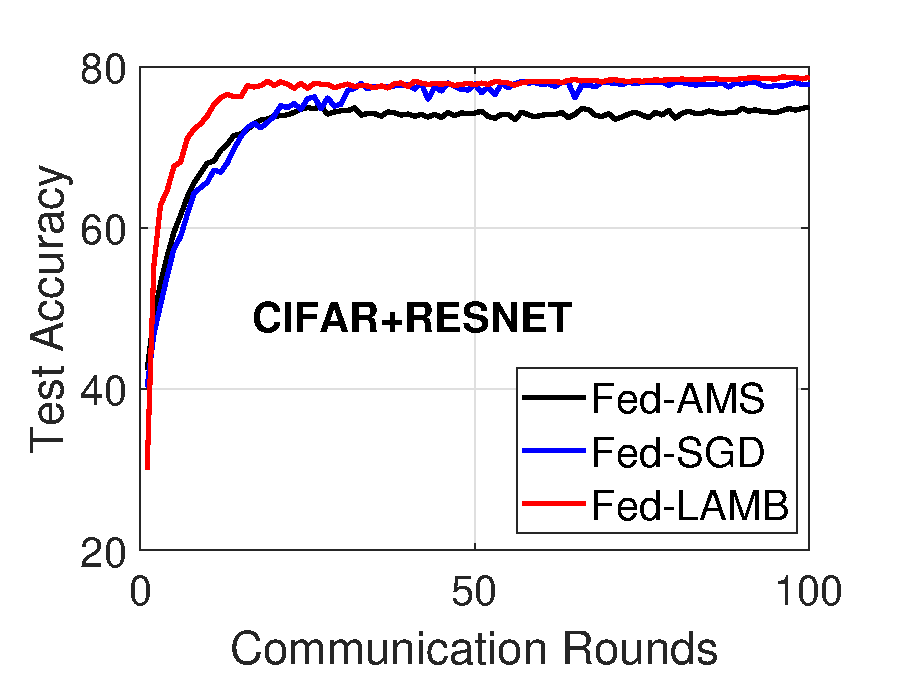
\includegraphics[width=0.5\textwidth]{figure/cifar_testerror_resnet_ep1_client10_iid1_SGD.eps}
                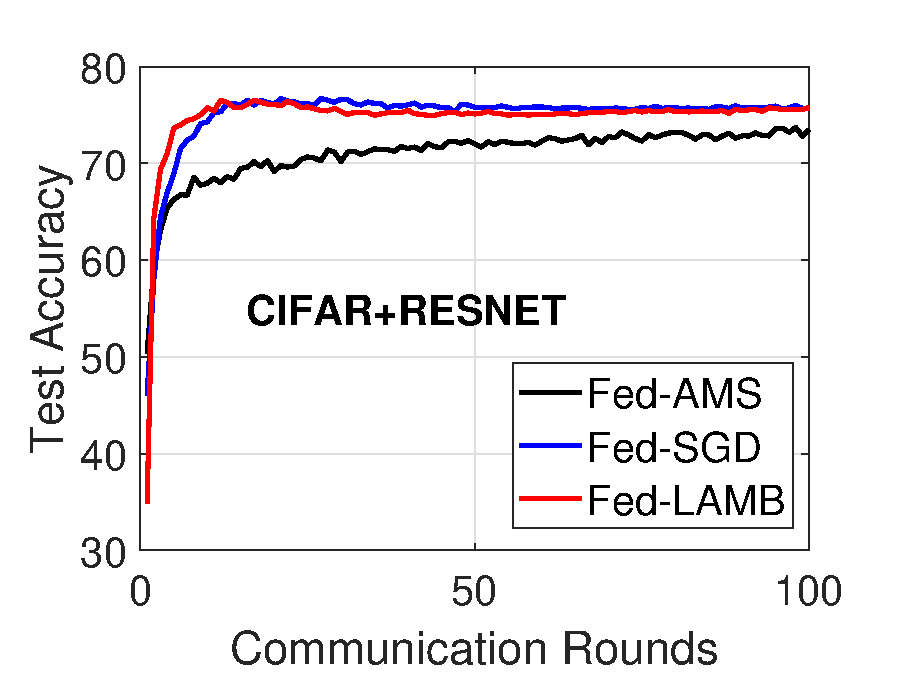
\includegraphics[width=0.5\textwidth]{figure/cifar_testerror_resnet_ep3_client10_iid1_SGD.eps}
        }
    \end{center}
	\caption{\textbf{From Left to Right}: Test accuracy on CIFAR+ResNet, with iid data distribution. 10 clients and (Left) 1 local epoch, (Right) 3 local epochs.}
	\label{fig:cifar-cnn-iid-bis}
\end{figure}


\end{document}    